% **************************************************************************************************************
% A Classic Thesis Style
% An Homage to The Elements of Typographic Style
%
% Copyright (C) 2017 André Miede and Ivo Pletikosić
%
% If you like the style then I would appreciate a postcard. My address
% can be found in the file ClassicThesis.pdf. A collection of the
% postcards I received so far is available online at
% http://postcards.miede.de
%
% License:
% This program is free software; you can redistribute it and/or modify
% it under the terms of the GNU General Public License as published by
% the Free Software Foundation; either version 2 of the License, or
% (at your option) any later version.
%
% This program is distributed in the hope that it will be useful,
% but WITHOUT ANY WARRANTY; without even the implied warranty of
% MERCHANTABILITY or FITNESS FOR A PARTICULAR PURPOSE.  See the
% GNU General Public License for more details.
%
% You should have received a copy of the GNU General Public License
% along with this program; see the file COPYING.  If not, write to
% the Free Software Foundation, Inc., 59 Temple Place - Suite 330,
% Boston, MA 02111-1307, USA.
%
% PLEASE SEE ALSO THE AUTHORS' NOTE REGARDING THIS LICENSE
% IN THE DOCUMENTATION (ClassicThesis.pdf --> Chapter 1 / Chapter01.tex)
% **************************************************************************************************************
\RequirePackage{silence} % :-\
    \WarningFilter{scrreprt}{Usage of package `titlesec'}
    %\WarningFilter{scrreprt}{Activating an ugly workaround}
    \WarningFilter{titlesec}{Non standard sectioning command detected}
\documentclass[ 
				oneside, % twoside
				openright,titlepage,numbers=noenddot,headinclude,%1headlines,% letterpaper a4paper
                footinclude=true,cleardoublepage=empty,abstractoff, % <--- obsolete, remove (todo)
                BCOR=5mm,paper=a4,fontsize=11pt,%11pt,a4paper,%
                czech,american,%
                ]{scrreprt}

%********************************************************************
% Note: Make all your adjustments in here
%*******************************************************
\usepackage{algorithm}
\usepackage{algorithmic}
\usepackage{amsthm}
\usepackage{datetime}


\newdateformat{monthyeardate}{\monthname[\THEMONTH], \THEYEAR}

\newcommand{\todo}[1]{\begingroup
            \color{Red} \textbf{todo:} {#1}
        	\endgroup }
        	
\newcommand{\unclear}[1]{\begingroup
            \color{Orange} \textbf{unclear:} {#1}
        	\endgroup }



\newcommand{\cvar}{\text{CVaR}}
\newcommand{\var}{\text{VaR}}

\newcommand{\envelope}{\mathcal{U}_{\cvar}(\alpha, P(\cdot | x, a))}



\newcommand{\indicator}{\mathbb{1}}
\renewcommand{\exp}{\mathbb{E}}
\newcommand{\expval}[1]{\mathbb{E}\left[ {#1} \right]}


%\newcommand{\exp}{\mathbb{E}}
\newcommand{\given}[1][]{\:#1\vert\:}

\newtheorem{theorem}{Theorem}
\newtheorem{corollary}{Corollary}
\newtheorem{lemma}{Lemma}



\newcommand{\bround}[1]{\left( {#1} \right)}
\newcommand{\bsquare}[1]{\left[ {#1} \right]}
\newcommand{\braces}[1]{\left{ {#1} \right}}




% ****************************************************************************************************
% classicthesis-config.tex
% formerly known as loadpackages.sty, classicthesis-ldpkg.sty, and classicthesis-preamble.sty
% Use it at the beginning of your ClassicThesis.tex, or as a LaTeX Preamble
% in your ClassicThesis.{tex,lyx} with % ****************************************************************************************************
% classicthesis-config.tex
% formerly known as loadpackages.sty, classicthesis-ldpkg.sty, and classicthesis-preamble.sty
% Use it at the beginning of your ClassicThesis.tex, or as a LaTeX Preamble
% in your ClassicThesis.{tex,lyx} with % ****************************************************************************************************
% classicthesis-config.tex
% formerly known as loadpackages.sty, classicthesis-ldpkg.sty, and classicthesis-preamble.sty
% Use it at the beginning of your ClassicThesis.tex, or as a LaTeX Preamble
% in your ClassicThesis.{tex,lyx} with \input{classicthesis-config}
% ****************************************************************************************************
% If you like the classicthesis, then I would appreciate a postcard.
% My address can be found in the file ClassicThesis.pdf. A collection
% of the postcards I received so far is available online at
% http://postcards.miede.de
% ****************************************************************************************************


% ****************************************************************************************************
% 0. Set the encoding of your files. UTF-8 is the only sensible encoding nowadays. If you can't read
% äöüßáéçèê∂åëæƒÏ€ then change the encoding setting in your editor, not the line below. If your editor
% does not support utf8 use another editor!
% ****************************************************************************************************
\PassOptionsToPackage{utf8}{inputenc}
  \usepackage{inputenc}

% ****************************************************************************************************
% 1. Configure classicthesis for your needs here, e.g., remove "drafting" below
% in order to deactivate the time-stamp on the pages
% (see ClassicThesis.pdf for more information):
% ****************************************************************************************************
\PassOptionsToPackage{
  drafting=false,    % print version information on the bottom of the pages
  tocaligned=false, % the left column of the toc will be aligned (no indentation)
  dottedtoc=false,  % page numbers in ToC flushed right
  parts=false,       % use part division
  eulerchapternumbers=true, % use AMS Euler for chapter font (otherwise Palatino)
  linedheaders=true,       % chapter headers will have line above and beneath
  floatperchapter=true,     % numbering per chapter for all floats (i.e., Figure 1.1)
  listings=true,    % load listings package and setup LoL
  subfig=true,      % setup for preloaded subfig package
  eulermath=false,  % use awesome Euler fonts for mathematical formulae (only with pdfLaTeX)
  beramono=false,    % toggle a nice monospaced font (w/ bold)
  minionpro=false   % setup for minion pro font; use minion pro small caps as well (only with pdfLaTeX)
}{classicthesis}


% ****************************************************************************************************
% 2. Personal data and user ad-hoc commands
% ****************************************************************************************************
\newcommand{\myTitle}{Risk-Averse Distributional Reinforcement Learning\xspace}
\newcommand{\mySubtitle}{a CVaR Optimization Approach\xspace}
\newcommand{\myDegree}{Engineer (Ing.)\xspace}
\newcommand{\myName}{Silvestr Stanko\xspace}
\newcommand{\myProf}{Put name here\xspace}
\newcommand{\myOtherProf}{Put name here\xspace}
\newcommand{\mySupervisor}{Put name here\xspace}
\newcommand{\myFaculty}{Faculty of Electrical Engineering\xspace}
\newcommand{\myDepartment}{Department of Computer Science\xspace}
\newcommand{\myUni}{Czech Technical University\xspace}
\newcommand{\myLocation}{Prague\xspace}
\newcommand{\myTime}{\monthyeardate\today\xspace}
\newcommand{\myVersion}{version 1.0}

% ********************************************************************
% Setup, finetuning, and useful commands
% ********************************************************************
\newcounter{dummy} % necessary for correct hyperlinks (to index, bib, etc.)
\newlength{\abcd} % for ab..z string length calculation
\providecommand{\mLyX}{L\kern-.1667em\lower.25em\hbox{Y}\kern-.125emX\@}
\newcommand{\ie}{i.\,e.}
\newcommand{\Ie}{I.\,e.}
\newcommand{\eg}{e.\,g.}
\newcommand{\Eg}{E.\,g.}
% ****************************************************************************************************


% ****************************************************************************************************
% 3. Loading some handy packages
% ****************************************************************************************************
% ********************************************************************
% Packages with options that might require adjustments
% ********************************************************************
%\PassOptionsToPackage{ngerman,american}{babel}   % change this to your language(s), main language last
% Spanish languages need extra options in order to work with this template
%\PassOptionsToPackage{spanish,es-lcroman}{babel}
    \usepackage{babel}

\usepackage{csquotes}
\PassOptionsToPackage{%
  %backend=biber,bibencoding=utf8, %instead of bibtex
  backend=bibtex8,bibencoding=ascii,%
  language=auto,%
  style=numeric-comp,%
  %style=authoryear-comp, % Author 1999, 2010
  %bibstyle=authoryear,dashed=false, % dashed: substitute rep. author with ---
  sorting=nyt, % name, year, title
  maxbibnames=10, % default: 3, et al.
  %backref=true,%
  natbib=true % natbib compatibility mode (\citep and \citet still work)
}{biblatex}
    \usepackage{biblatex}

\PassOptionsToPackage{fleqn}{amsmath}       % math environments and more by the AMS
  \usepackage{amsmath}

% ********************************************************************
% General useful packages
% ********************************************************************
\PassOptionsToPackage{T1}{fontenc} % T2A for cyrillics
  \usepackage{fontenc}
\usepackage{textcomp} % fix warning with missing font shapes
\usepackage{scrhack} % fix warnings when using KOMA with listings package
\usepackage{xspace} % to get the spacing after macros right
\usepackage{mparhack} % get marginpar right
%\usepackage{fixltx2e} % fixes some LaTeX stuff --> since 2015 in the LaTeX kernel (see below)
% \usepackage[latest]{latexrelease} % emulate newer kernel version if older is detected
\PassOptionsToPackage{printonlyused,smaller}{acronym}
  \usepackage{acronym} % nice macros for handling all acronyms in the thesis
  %\renewcommand{\bflabel}[1]{{#1}\hfill} % fix the list of acronyms --> no longer working
  %\renewcommand*{\acsfont}[1]{\textsc{#1}}
  %\renewcommand*{\aclabelfont}[1]{\acsfont{#1}}
  %\def\bflabel#1{{#1\hfill}}
  \def\bflabel#1{{\acsfont{#1}\hfill}}
  \def\aclabelfont#1{\acsfont{#1}}
% ****************************************************************************************************
%\usepackage{pgfplots} % External TikZ/PGF support (thanks to Andreas Nautsch)
%\usetikzlibrary{external}
%\tikzexternalize[mode=list and make, prefix=ext-tikz/]
% ****************************************************************************************************


% ****************************************************************************************************
% 4. Setup floats: tables, (sub)figures, and captions
% ****************************************************************************************************
\usepackage{tabularx} % better tables
  \setlength{\extrarowheight}{3pt} % increase table row height
\newcommand{\tableheadline}[1]{\multicolumn{1}{c}{\spacedlowsmallcaps{#1}}}
\newcommand{\myfloatalign}{\centering} % to be used with each float for alignment
\usepackage{caption}
% Thanks to cgnieder and Claus Lahiri
% http://tex.stackexchange.com/questions/69349/spacedlowsmallcaps-in-caption-label
% [REMOVED DUE TO OTHER PROBLEMS, SEE ISSUE #82]
%\DeclareCaptionLabelFormat{smallcaps}{\bothIfFirst{#1}{~}\MakeTextLowercase{\textsc{#2}}}
%\captionsetup{font=small,labelformat=smallcaps} % format=hang,
\captionsetup{font=small} % format=hang,
\usepackage{subfig}
% ****************************************************************************************************


% ****************************************************************************************************
% 5. Setup code listings
% ****************************************************************************************************
\usepackage{listings}
%\lstset{emph={trueIndex,root},emphstyle=\color{BlueViolet}}%\underbar} % for special keywords
\lstset{language=[LaTeX]Tex,%C++,
  morekeywords={PassOptionsToPackage,selectlanguage},
  keywordstyle=\color{RoyalBlue},%\bfseries,
  basicstyle=\small\ttfamily,
  %identifierstyle=\color{NavyBlue},
  commentstyle=\color{Green}\ttfamily,
  stringstyle=\rmfamily,
  numbers=none,%left,%
  numberstyle=\scriptsize,%\tiny
  stepnumber=5,
  numbersep=8pt,
  showstringspaces=false,
  breaklines=true,
  %frameround=ftff,
  %frame=single,
  belowcaptionskip=.75\baselineskip
  %frame=L
}
% ****************************************************************************************************


% ****************************************************************************************************
% 6. PDFLaTeX, hyperreferences, and citation backreferences
% ****************************************************************************************************
% ********************************************************************
% Using PDFLaTeX
% ********************************************************************
\PassOptionsToPackage{hyperfootnotes=false,pdfpagelabels}{hyperref}
  \usepackage{hyperref}  % backref linktocpage pagebackref
%\ifpdf
%\pdfcompresslevel=9
%\pdfadjustspacing=1
%\fi
%\PassOptionsToPackage{pdftex}{graphicx} %%%IVO: driver will be chosen automatically
  \usepackage{graphicx}


% ********************************************************************
% Hyperreferences
% ********************************************************************
\hypersetup{%
  %draft, % hyperref's draft mode, for printing see below
  colorlinks=true, linktocpage=true, pdfstartpage=3, pdfstartview=FitV,%
  % uncomment the following line if you want to have black links (e.g., for printing)
  %colorlinks=false, linktocpage=false, pdfstartpage=3, pdfstartview=FitV, pdfborder={0 0 0},%
  breaklinks=true, pdfpagemode=UseNone, pageanchor=true, pdfpagemode=UseOutlines,%
  plainpages=false, bookmarksnumbered, bookmarksopen=true, bookmarksopenlevel=1,%
  hypertexnames=true, pdfhighlight=/O,%nesting=true,%frenchlinks,%
  urlcolor=webbrown, linkcolor=RoyalBlue, citecolor=webgreen, %pagecolor=RoyalBlue,%
  %urlcolor=Black, linkcolor=Black, citecolor=Black, %pagecolor=Black,%
  pdftitle={\myTitle},%
  pdfauthor={\textcopyright\ \myName, \myUni, \myFaculty},%
  pdfsubject={},%
  pdfkeywords={},%
  pdfcreator={pdfLaTeX},%
  pdfproducer={LaTeX with hyperref and classicthesis}%
}

% ********************************************************************
% Setup autoreferences
% ********************************************************************
% There are some issues regarding autorefnames
% http://www.ureader.de/msg/136221647.aspx
% http://www.tex.ac.uk/cgi-bin/texfaq2html?label=latexwords
% you have to redefine the makros for the
% language you use, e.g., american, ngerman
% (as chosen when loading babel/AtBeginDocument)
% ********************************************************************
\makeatletter
\@ifpackageloaded{babel}%
  {%
    \addto\extrasamerican{%
      \renewcommand*{\figureautorefname}{Figure}%
      \renewcommand*{\tableautorefname}{Table}%
      \renewcommand*{\partautorefname}{Part}%
      \renewcommand*{\chapterautorefname}{Chapter}%
      \renewcommand*{\sectionautorefname}{Section}%
      \renewcommand*{\subsectionautorefname}{Section}%
      \renewcommand*{\subsubsectionautorefname}{Section}%
    }%
%    \addto\extrasngerman{%
%      \renewcommand*{\paragraphautorefname}{Absatz}%
%      \renewcommand*{\subparagraphautorefname}{Unterabsatz}%
%      \renewcommand*{\footnoteautorefname}{Fu\"snote}%
%      \renewcommand*{\FancyVerbLineautorefname}{Zeile}%
%      \renewcommand*{\theoremautorefname}{Theorem}%
%      \renewcommand*{\appendixautorefname}{Anhang}%
%      \renewcommand*{\equationautorefname}{Gleichung}%
%      \renewcommand*{\itemautorefname}{Punkt}%
%    }%
      % Fix to getting autorefs for subfigures right (thanks to Belinda Vogt for changing the definition)
      \providecommand{\subfigureautorefname}{\figureautorefname}%
    }{\relax}
\makeatother


% ****************************************************************************************************
% 7. Last calls before the bar closes
% ****************************************************************************************************
% ********************************************************************
% Development Stuff
% ********************************************************************
\listfiles
%\PassOptionsToPackage{l2tabu,orthodox,abort}{nag}
%  \usepackage{nag}
%\PassOptionsToPackage{warning, all}{onlyamsmath}
%  \usepackage{onlyamsmath}

% ********************************************************************
% Last, but not least...
% ********************************************************************
\usepackage{classicthesis}
% ****************************************************************************************************


% ****************************************************************************************************
% 8. Further adjustments (experimental)
% ****************************************************************************************************
% ********************************************************************
% Changing the text area
% ********************************************************************
\areaset[current]{400pt}{761pt} % 686 (factor 2.2) + 33 head + 42 head \the\footskip
%\setlength{\marginparwidth}{7em}%
%\setlength{\marginparsep}{2em}%

% ********************************************************************
% Using different fonts
% ********************************************************************
%\usepackage[oldstylenums]{kpfonts} % oldstyle notextcomp
%\usepackage[osf]{libertine}
%\usepackage[light,condensed,math]{iwona}
%\renewcommand{\sfdefault}{iwona}
\usepackage{lmodern} % <-- no osf support :-(
%\usepackage{cfr-lm} %
%\usepackage[urw-garamond]{mathdesign} <-- no osf support :-(
%\usepackage[default,osfigures]{opensans} % scale=0.95
%\usepackage[sfdefault]{FiraSans}
% ********************************************************************
% \usepackage[largesc,osf]{newpxtext}
% Used to fix these:
% https://bitbucket.org/amiede/classicthesis/issues/139/italics-in-pallatino-capitals-chapter
% https://bitbucket.org/amiede/classicthesis/issues/45/problema-testatine-su-classicthesis-style
% ********************************************************************
%\linespread{1.05} % a bit more for Palatino
% ****************************************************************************************************

% ****************************************************************************************************
% If you like the classicthesis, then I would appreciate a postcard.
% My address can be found in the file ClassicThesis.pdf. A collection
% of the postcards I received so far is available online at
% http://postcards.miede.de
% ****************************************************************************************************


% ****************************************************************************************************
% 0. Set the encoding of your files. UTF-8 is the only sensible encoding nowadays. If you can't read
% äöüßáéçèê∂åëæƒÏ€ then change the encoding setting in your editor, not the line below. If your editor
% does not support utf8 use another editor!
% ****************************************************************************************************
\PassOptionsToPackage{utf8}{inputenc}
  \usepackage{inputenc}

% ****************************************************************************************************
% 1. Configure classicthesis for your needs here, e.g., remove "drafting" below
% in order to deactivate the time-stamp on the pages
% (see ClassicThesis.pdf for more information):
% ****************************************************************************************************
\PassOptionsToPackage{
  drafting=false,    % print version information on the bottom of the pages
  tocaligned=false, % the left column of the toc will be aligned (no indentation)
  dottedtoc=false,  % page numbers in ToC flushed right
  parts=false,       % use part division
  eulerchapternumbers=true, % use AMS Euler for chapter font (otherwise Palatino)
  linedheaders=true,       % chapter headers will have line above and beneath
  floatperchapter=true,     % numbering per chapter for all floats (i.e., Figure 1.1)
  listings=true,    % load listings package and setup LoL
  subfig=true,      % setup for preloaded subfig package
  eulermath=false,  % use awesome Euler fonts for mathematical formulae (only with pdfLaTeX)
  beramono=false,    % toggle a nice monospaced font (w/ bold)
  minionpro=false   % setup for minion pro font; use minion pro small caps as well (only with pdfLaTeX)
}{classicthesis}


% ****************************************************************************************************
% 2. Personal data and user ad-hoc commands
% ****************************************************************************************************
\newcommand{\myTitle}{Risk-Averse Distributional Reinforcement Learning\xspace}
\newcommand{\mySubtitle}{a CVaR Optimization Approach\xspace}
\newcommand{\myDegree}{Engineer (Ing.)\xspace}
\newcommand{\myName}{Silvestr Stanko\xspace}
\newcommand{\myProf}{Put name here\xspace}
\newcommand{\myOtherProf}{Put name here\xspace}
\newcommand{\mySupervisor}{Put name here\xspace}
\newcommand{\myFaculty}{Faculty of Electrical Engineering\xspace}
\newcommand{\myDepartment}{Department of Computer Science\xspace}
\newcommand{\myUni}{Czech Technical University\xspace}
\newcommand{\myLocation}{Prague\xspace}
\newcommand{\myTime}{\monthyeardate\today\xspace}
\newcommand{\myVersion}{version 1.0}

% ********************************************************************
% Setup, finetuning, and useful commands
% ********************************************************************
\newcounter{dummy} % necessary for correct hyperlinks (to index, bib, etc.)
\newlength{\abcd} % for ab..z string length calculation
\providecommand{\mLyX}{L\kern-.1667em\lower.25em\hbox{Y}\kern-.125emX\@}
\newcommand{\ie}{i.\,e.}
\newcommand{\Ie}{I.\,e.}
\newcommand{\eg}{e.\,g.}
\newcommand{\Eg}{E.\,g.}
% ****************************************************************************************************


% ****************************************************************************************************
% 3. Loading some handy packages
% ****************************************************************************************************
% ********************************************************************
% Packages with options that might require adjustments
% ********************************************************************
%\PassOptionsToPackage{ngerman,american}{babel}   % change this to your language(s), main language last
% Spanish languages need extra options in order to work with this template
%\PassOptionsToPackage{spanish,es-lcroman}{babel}
    \usepackage{babel}

\usepackage{csquotes}
\PassOptionsToPackage{%
  %backend=biber,bibencoding=utf8, %instead of bibtex
  backend=bibtex8,bibencoding=ascii,%
  language=auto,%
  style=numeric-comp,%
  %style=authoryear-comp, % Author 1999, 2010
  %bibstyle=authoryear,dashed=false, % dashed: substitute rep. author with ---
  sorting=nyt, % name, year, title
  maxbibnames=10, % default: 3, et al.
  %backref=true,%
  natbib=true % natbib compatibility mode (\citep and \citet still work)
}{biblatex}
    \usepackage{biblatex}

\PassOptionsToPackage{fleqn}{amsmath}       % math environments and more by the AMS
  \usepackage{amsmath}

% ********************************************************************
% General useful packages
% ********************************************************************
\PassOptionsToPackage{T1}{fontenc} % T2A for cyrillics
  \usepackage{fontenc}
\usepackage{textcomp} % fix warning with missing font shapes
\usepackage{scrhack} % fix warnings when using KOMA with listings package
\usepackage{xspace} % to get the spacing after macros right
\usepackage{mparhack} % get marginpar right
%\usepackage{fixltx2e} % fixes some LaTeX stuff --> since 2015 in the LaTeX kernel (see below)
% \usepackage[latest]{latexrelease} % emulate newer kernel version if older is detected
\PassOptionsToPackage{printonlyused,smaller}{acronym}
  \usepackage{acronym} % nice macros for handling all acronyms in the thesis
  %\renewcommand{\bflabel}[1]{{#1}\hfill} % fix the list of acronyms --> no longer working
  %\renewcommand*{\acsfont}[1]{\textsc{#1}}
  %\renewcommand*{\aclabelfont}[1]{\acsfont{#1}}
  %\def\bflabel#1{{#1\hfill}}
  \def\bflabel#1{{\acsfont{#1}\hfill}}
  \def\aclabelfont#1{\acsfont{#1}}
% ****************************************************************************************************
%\usepackage{pgfplots} % External TikZ/PGF support (thanks to Andreas Nautsch)
%\usetikzlibrary{external}
%\tikzexternalize[mode=list and make, prefix=ext-tikz/]
% ****************************************************************************************************


% ****************************************************************************************************
% 4. Setup floats: tables, (sub)figures, and captions
% ****************************************************************************************************
\usepackage{tabularx} % better tables
  \setlength{\extrarowheight}{3pt} % increase table row height
\newcommand{\tableheadline}[1]{\multicolumn{1}{c}{\spacedlowsmallcaps{#1}}}
\newcommand{\myfloatalign}{\centering} % to be used with each float for alignment
\usepackage{caption}
% Thanks to cgnieder and Claus Lahiri
% http://tex.stackexchange.com/questions/69349/spacedlowsmallcaps-in-caption-label
% [REMOVED DUE TO OTHER PROBLEMS, SEE ISSUE #82]
%\DeclareCaptionLabelFormat{smallcaps}{\bothIfFirst{#1}{~}\MakeTextLowercase{\textsc{#2}}}
%\captionsetup{font=small,labelformat=smallcaps} % format=hang,
\captionsetup{font=small} % format=hang,
\usepackage{subfig}
% ****************************************************************************************************


% ****************************************************************************************************
% 5. Setup code listings
% ****************************************************************************************************
\usepackage{listings}
%\lstset{emph={trueIndex,root},emphstyle=\color{BlueViolet}}%\underbar} % for special keywords
\lstset{language=[LaTeX]Tex,%C++,
  morekeywords={PassOptionsToPackage,selectlanguage},
  keywordstyle=\color{RoyalBlue},%\bfseries,
  basicstyle=\small\ttfamily,
  %identifierstyle=\color{NavyBlue},
  commentstyle=\color{Green}\ttfamily,
  stringstyle=\rmfamily,
  numbers=none,%left,%
  numberstyle=\scriptsize,%\tiny
  stepnumber=5,
  numbersep=8pt,
  showstringspaces=false,
  breaklines=true,
  %frameround=ftff,
  %frame=single,
  belowcaptionskip=.75\baselineskip
  %frame=L
}
% ****************************************************************************************************


% ****************************************************************************************************
% 6. PDFLaTeX, hyperreferences, and citation backreferences
% ****************************************************************************************************
% ********************************************************************
% Using PDFLaTeX
% ********************************************************************
\PassOptionsToPackage{hyperfootnotes=false,pdfpagelabels}{hyperref}
  \usepackage{hyperref}  % backref linktocpage pagebackref
%\ifpdf
%\pdfcompresslevel=9
%\pdfadjustspacing=1
%\fi
%\PassOptionsToPackage{pdftex}{graphicx} %%%IVO: driver will be chosen automatically
  \usepackage{graphicx}


% ********************************************************************
% Hyperreferences
% ********************************************************************
\hypersetup{%
  %draft, % hyperref's draft mode, for printing see below
  colorlinks=true, linktocpage=true, pdfstartpage=3, pdfstartview=FitV,%
  % uncomment the following line if you want to have black links (e.g., for printing)
  %colorlinks=false, linktocpage=false, pdfstartpage=3, pdfstartview=FitV, pdfborder={0 0 0},%
  breaklinks=true, pdfpagemode=UseNone, pageanchor=true, pdfpagemode=UseOutlines,%
  plainpages=false, bookmarksnumbered, bookmarksopen=true, bookmarksopenlevel=1,%
  hypertexnames=true, pdfhighlight=/O,%nesting=true,%frenchlinks,%
  urlcolor=webbrown, linkcolor=RoyalBlue, citecolor=webgreen, %pagecolor=RoyalBlue,%
  %urlcolor=Black, linkcolor=Black, citecolor=Black, %pagecolor=Black,%
  pdftitle={\myTitle},%
  pdfauthor={\textcopyright\ \myName, \myUni, \myFaculty},%
  pdfsubject={},%
  pdfkeywords={},%
  pdfcreator={pdfLaTeX},%
  pdfproducer={LaTeX with hyperref and classicthesis}%
}

% ********************************************************************
% Setup autoreferences
% ********************************************************************
% There are some issues regarding autorefnames
% http://www.ureader.de/msg/136221647.aspx
% http://www.tex.ac.uk/cgi-bin/texfaq2html?label=latexwords
% you have to redefine the makros for the
% language you use, e.g., american, ngerman
% (as chosen when loading babel/AtBeginDocument)
% ********************************************************************
\makeatletter
\@ifpackageloaded{babel}%
  {%
    \addto\extrasamerican{%
      \renewcommand*{\figureautorefname}{Figure}%
      \renewcommand*{\tableautorefname}{Table}%
      \renewcommand*{\partautorefname}{Part}%
      \renewcommand*{\chapterautorefname}{Chapter}%
      \renewcommand*{\sectionautorefname}{Section}%
      \renewcommand*{\subsectionautorefname}{Section}%
      \renewcommand*{\subsubsectionautorefname}{Section}%
    }%
%    \addto\extrasngerman{%
%      \renewcommand*{\paragraphautorefname}{Absatz}%
%      \renewcommand*{\subparagraphautorefname}{Unterabsatz}%
%      \renewcommand*{\footnoteautorefname}{Fu\"snote}%
%      \renewcommand*{\FancyVerbLineautorefname}{Zeile}%
%      \renewcommand*{\theoremautorefname}{Theorem}%
%      \renewcommand*{\appendixautorefname}{Anhang}%
%      \renewcommand*{\equationautorefname}{Gleichung}%
%      \renewcommand*{\itemautorefname}{Punkt}%
%    }%
      % Fix to getting autorefs for subfigures right (thanks to Belinda Vogt for changing the definition)
      \providecommand{\subfigureautorefname}{\figureautorefname}%
    }{\relax}
\makeatother


% ****************************************************************************************************
% 7. Last calls before the bar closes
% ****************************************************************************************************
% ********************************************************************
% Development Stuff
% ********************************************************************
\listfiles
%\PassOptionsToPackage{l2tabu,orthodox,abort}{nag}
%  \usepackage{nag}
%\PassOptionsToPackage{warning, all}{onlyamsmath}
%  \usepackage{onlyamsmath}

% ********************************************************************
% Last, but not least...
% ********************************************************************
\usepackage{classicthesis}
% ****************************************************************************************************


% ****************************************************************************************************
% 8. Further adjustments (experimental)
% ****************************************************************************************************
% ********************************************************************
% Changing the text area
% ********************************************************************
\areaset[current]{400pt}{761pt} % 686 (factor 2.2) + 33 head + 42 head \the\footskip
%\setlength{\marginparwidth}{7em}%
%\setlength{\marginparsep}{2em}%

% ********************************************************************
% Using different fonts
% ********************************************************************
%\usepackage[oldstylenums]{kpfonts} % oldstyle notextcomp
%\usepackage[osf]{libertine}
%\usepackage[light,condensed,math]{iwona}
%\renewcommand{\sfdefault}{iwona}
\usepackage{lmodern} % <-- no osf support :-(
%\usepackage{cfr-lm} %
%\usepackage[urw-garamond]{mathdesign} <-- no osf support :-(
%\usepackage[default,osfigures]{opensans} % scale=0.95
%\usepackage[sfdefault]{FiraSans}
% ********************************************************************
% \usepackage[largesc,osf]{newpxtext}
% Used to fix these:
% https://bitbucket.org/amiede/classicthesis/issues/139/italics-in-pallatino-capitals-chapter
% https://bitbucket.org/amiede/classicthesis/issues/45/problema-testatine-su-classicthesis-style
% ********************************************************************
%\linespread{1.05} % a bit more for Palatino
% ****************************************************************************************************

% ****************************************************************************************************
% If you like the classicthesis, then I would appreciate a postcard.
% My address can be found in the file ClassicThesis.pdf. A collection
% of the postcards I received so far is available online at
% http://postcards.miede.de
% ****************************************************************************************************


% ****************************************************************************************************
% 0. Set the encoding of your files. UTF-8 is the only sensible encoding nowadays. If you can't read
% äöüßáéçèê∂åëæƒÏ€ then change the encoding setting in your editor, not the line below. If your editor
% does not support utf8 use another editor!
% ****************************************************************************************************
\PassOptionsToPackage{utf8}{inputenc}
  \usepackage{inputenc}

% ****************************************************************************************************
% 1. Configure classicthesis for your needs here, e.g., remove "drafting" below
% in order to deactivate the time-stamp on the pages
% (see ClassicThesis.pdf for more information):
% ****************************************************************************************************
\PassOptionsToPackage{
  drafting=false,    % print version information on the bottom of the pages
  tocaligned=false, % the left column of the toc will be aligned (no indentation)
  dottedtoc=false,  % page numbers in ToC flushed right
  parts=false,       % use part division
  eulerchapternumbers=true, % use AMS Euler for chapter font (otherwise Palatino)
  linedheaders=true,       % chapter headers will have line above and beneath
  floatperchapter=true,     % numbering per chapter for all floats (i.e., Figure 1.1)
  listings=true,    % load listings package and setup LoL
  subfig=true,      % setup for preloaded subfig package
  eulermath=false,  % use awesome Euler fonts for mathematical formulae (only with pdfLaTeX)
  beramono=false,    % toggle a nice monospaced font (w/ bold)
  minionpro=false   % setup for minion pro font; use minion pro small caps as well (only with pdfLaTeX)
}{classicthesis}


% ****************************************************************************************************
% 2. Personal data and user ad-hoc commands
% ****************************************************************************************************
\newcommand{\myTitle}{Risk-Averse Distributional Reinforcement Learning\xspace}
\newcommand{\mySubtitle}{a CVaR Optimization Approach\xspace}
\newcommand{\myDegree}{Engineer (Ing.)\xspace}
\newcommand{\myName}{Silvestr Stanko\xspace}
\newcommand{\myProf}{Put name here\xspace}
\newcommand{\myOtherProf}{Put name here\xspace}
\newcommand{\mySupervisor}{Put name here\xspace}
\newcommand{\myFaculty}{Faculty of Electrical Engineering\xspace}
\newcommand{\myDepartment}{Department of Computer Science\xspace}
\newcommand{\myUni}{Czech Technical University\xspace}
\newcommand{\myLocation}{Prague\xspace}
\newcommand{\myTime}{\monthyeardate\today\xspace}
\newcommand{\myVersion}{version 1.0}

% ********************************************************************
% Setup, finetuning, and useful commands
% ********************************************************************
\newcounter{dummy} % necessary for correct hyperlinks (to index, bib, etc.)
\newlength{\abcd} % for ab..z string length calculation
\providecommand{\mLyX}{L\kern-.1667em\lower.25em\hbox{Y}\kern-.125emX\@}
\newcommand{\ie}{i.\,e.}
\newcommand{\Ie}{I.\,e.}
\newcommand{\eg}{e.\,g.}
\newcommand{\Eg}{E.\,g.}
% ****************************************************************************************************


% ****************************************************************************************************
% 3. Loading some handy packages
% ****************************************************************************************************
% ********************************************************************
% Packages with options that might require adjustments
% ********************************************************************
%\PassOptionsToPackage{ngerman,american}{babel}   % change this to your language(s), main language last
% Spanish languages need extra options in order to work with this template
%\PassOptionsToPackage{spanish,es-lcroman}{babel}
    \usepackage{babel}

\usepackage{csquotes}
\PassOptionsToPackage{%
  %backend=biber,bibencoding=utf8, %instead of bibtex
  backend=bibtex8,bibencoding=ascii,%
  language=auto,%
  style=numeric-comp,%
  %style=authoryear-comp, % Author 1999, 2010
  %bibstyle=authoryear,dashed=false, % dashed: substitute rep. author with ---
  sorting=nyt, % name, year, title
  maxbibnames=10, % default: 3, et al.
  %backref=true,%
  natbib=true % natbib compatibility mode (\citep and \citet still work)
}{biblatex}
    \usepackage{biblatex}

\PassOptionsToPackage{fleqn}{amsmath}       % math environments and more by the AMS
  \usepackage{amsmath}

% ********************************************************************
% General useful packages
% ********************************************************************
\PassOptionsToPackage{T1}{fontenc} % T2A for cyrillics
  \usepackage{fontenc}
\usepackage{textcomp} % fix warning with missing font shapes
\usepackage{scrhack} % fix warnings when using KOMA with listings package
\usepackage{xspace} % to get the spacing after macros right
\usepackage{mparhack} % get marginpar right
%\usepackage{fixltx2e} % fixes some LaTeX stuff --> since 2015 in the LaTeX kernel (see below)
% \usepackage[latest]{latexrelease} % emulate newer kernel version if older is detected
\PassOptionsToPackage{printonlyused,smaller}{acronym}
  \usepackage{acronym} % nice macros for handling all acronyms in the thesis
  %\renewcommand{\bflabel}[1]{{#1}\hfill} % fix the list of acronyms --> no longer working
  %\renewcommand*{\acsfont}[1]{\textsc{#1}}
  %\renewcommand*{\aclabelfont}[1]{\acsfont{#1}}
  %\def\bflabel#1{{#1\hfill}}
  \def\bflabel#1{{\acsfont{#1}\hfill}}
  \def\aclabelfont#1{\acsfont{#1}}
% ****************************************************************************************************
%\usepackage{pgfplots} % External TikZ/PGF support (thanks to Andreas Nautsch)
%\usetikzlibrary{external}
%\tikzexternalize[mode=list and make, prefix=ext-tikz/]
% ****************************************************************************************************


% ****************************************************************************************************
% 4. Setup floats: tables, (sub)figures, and captions
% ****************************************************************************************************
\usepackage{tabularx} % better tables
  \setlength{\extrarowheight}{3pt} % increase table row height
\newcommand{\tableheadline}[1]{\multicolumn{1}{c}{\spacedlowsmallcaps{#1}}}
\newcommand{\myfloatalign}{\centering} % to be used with each float for alignment
\usepackage{caption}
% Thanks to cgnieder and Claus Lahiri
% http://tex.stackexchange.com/questions/69349/spacedlowsmallcaps-in-caption-label
% [REMOVED DUE TO OTHER PROBLEMS, SEE ISSUE #82]
%\DeclareCaptionLabelFormat{smallcaps}{\bothIfFirst{#1}{~}\MakeTextLowercase{\textsc{#2}}}
%\captionsetup{font=small,labelformat=smallcaps} % format=hang,
\captionsetup{font=small} % format=hang,
\usepackage{subfig}
% ****************************************************************************************************


% ****************************************************************************************************
% 5. Setup code listings
% ****************************************************************************************************
\usepackage{listings}
%\lstset{emph={trueIndex,root},emphstyle=\color{BlueViolet}}%\underbar} % for special keywords
\lstset{language=[LaTeX]Tex,%C++,
  morekeywords={PassOptionsToPackage,selectlanguage},
  keywordstyle=\color{RoyalBlue},%\bfseries,
  basicstyle=\small\ttfamily,
  %identifierstyle=\color{NavyBlue},
  commentstyle=\color{Green}\ttfamily,
  stringstyle=\rmfamily,
  numbers=none,%left,%
  numberstyle=\scriptsize,%\tiny
  stepnumber=5,
  numbersep=8pt,
  showstringspaces=false,
  breaklines=true,
  %frameround=ftff,
  %frame=single,
  belowcaptionskip=.75\baselineskip
  %frame=L
}
% ****************************************************************************************************


% ****************************************************************************************************
% 6. PDFLaTeX, hyperreferences, and citation backreferences
% ****************************************************************************************************
% ********************************************************************
% Using PDFLaTeX
% ********************************************************************
\PassOptionsToPackage{hyperfootnotes=false,pdfpagelabels}{hyperref}
  \usepackage{hyperref}  % backref linktocpage pagebackref
%\ifpdf
%\pdfcompresslevel=9
%\pdfadjustspacing=1
%\fi
%\PassOptionsToPackage{pdftex}{graphicx} %%%IVO: driver will be chosen automatically
  \usepackage{graphicx}


% ********************************************************************
% Hyperreferences
% ********************************************************************
\hypersetup{%
  %draft, % hyperref's draft mode, for printing see below
  colorlinks=true, linktocpage=true, pdfstartpage=3, pdfstartview=FitV,%
  % uncomment the following line if you want to have black links (e.g., for printing)
  %colorlinks=false, linktocpage=false, pdfstartpage=3, pdfstartview=FitV, pdfborder={0 0 0},%
  breaklinks=true, pdfpagemode=UseNone, pageanchor=true, pdfpagemode=UseOutlines,%
  plainpages=false, bookmarksnumbered, bookmarksopen=true, bookmarksopenlevel=1,%
  hypertexnames=true, pdfhighlight=/O,%nesting=true,%frenchlinks,%
  urlcolor=webbrown, linkcolor=RoyalBlue, citecolor=webgreen, %pagecolor=RoyalBlue,%
  %urlcolor=Black, linkcolor=Black, citecolor=Black, %pagecolor=Black,%
  pdftitle={\myTitle},%
  pdfauthor={\textcopyright\ \myName, \myUni, \myFaculty},%
  pdfsubject={},%
  pdfkeywords={},%
  pdfcreator={pdfLaTeX},%
  pdfproducer={LaTeX with hyperref and classicthesis}%
}

% ********************************************************************
% Setup autoreferences
% ********************************************************************
% There are some issues regarding autorefnames
% http://www.ureader.de/msg/136221647.aspx
% http://www.tex.ac.uk/cgi-bin/texfaq2html?label=latexwords
% you have to redefine the makros for the
% language you use, e.g., american, ngerman
% (as chosen when loading babel/AtBeginDocument)
% ********************************************************************
\makeatletter
\@ifpackageloaded{babel}%
  {%
    \addto\extrasamerican{%
      \renewcommand*{\figureautorefname}{Figure}%
      \renewcommand*{\tableautorefname}{Table}%
      \renewcommand*{\partautorefname}{Part}%
      \renewcommand*{\chapterautorefname}{Chapter}%
      \renewcommand*{\sectionautorefname}{Section}%
      \renewcommand*{\subsectionautorefname}{Section}%
      \renewcommand*{\subsubsectionautorefname}{Section}%
    }%
%    \addto\extrasngerman{%
%      \renewcommand*{\paragraphautorefname}{Absatz}%
%      \renewcommand*{\subparagraphautorefname}{Unterabsatz}%
%      \renewcommand*{\footnoteautorefname}{Fu\"snote}%
%      \renewcommand*{\FancyVerbLineautorefname}{Zeile}%
%      \renewcommand*{\theoremautorefname}{Theorem}%
%      \renewcommand*{\appendixautorefname}{Anhang}%
%      \renewcommand*{\equationautorefname}{Gleichung}%
%      \renewcommand*{\itemautorefname}{Punkt}%
%    }%
      % Fix to getting autorefs for subfigures right (thanks to Belinda Vogt for changing the definition)
      \providecommand{\subfigureautorefname}{\figureautorefname}%
    }{\relax}
\makeatother


% ****************************************************************************************************
% 7. Last calls before the bar closes
% ****************************************************************************************************
% ********************************************************************
% Development Stuff
% ********************************************************************
\listfiles
%\PassOptionsToPackage{l2tabu,orthodox,abort}{nag}
%  \usepackage{nag}
%\PassOptionsToPackage{warning, all}{onlyamsmath}
%  \usepackage{onlyamsmath}

% ********************************************************************
% Last, but not least...
% ********************************************************************
\usepackage{classicthesis}
% ****************************************************************************************************


% ****************************************************************************************************
% 8. Further adjustments (experimental)
% ****************************************************************************************************
% ********************************************************************
% Changing the text area
% ********************************************************************
\areaset[current]{400pt}{761pt} % 686 (factor 2.2) + 33 head + 42 head \the\footskip
%\setlength{\marginparwidth}{7em}%
%\setlength{\marginparsep}{2em}%

% ********************************************************************
% Using different fonts
% ********************************************************************
%\usepackage[oldstylenums]{kpfonts} % oldstyle notextcomp
%\usepackage[osf]{libertine}
%\usepackage[light,condensed,math]{iwona}
%\renewcommand{\sfdefault}{iwona}
\usepackage{lmodern} % <-- no osf support :-(
%\usepackage{cfr-lm} %
%\usepackage[urw-garamond]{mathdesign} <-- no osf support :-(
%\usepackage[default,osfigures]{opensans} % scale=0.95
%\usepackage[sfdefault]{FiraSans}
% ********************************************************************
% \usepackage[largesc,osf]{newpxtext}
% Used to fix these:
% https://bitbucket.org/amiede/classicthesis/issues/139/italics-in-pallatino-capitals-chapter
% https://bitbucket.org/amiede/classicthesis/issues/45/problema-testatine-su-classicthesis-style
% ********************************************************************
%\linespread{1.05} % a bit more for Palatino
% ****************************************************************************************************



%\SetSymbolFont{operators}   {normal}{OT1}{cmr} {m}{n}
%\SetSymbolFont{letters}     {normal}{OML}{cmm} {m}{it}
%\SetSymbolFont{symbols}     {normal}{OMS}{cmsy}{m}{n}
%\SetSymbolFont{largesymbols}{normal}{OMX}{cmex}{m}{n}
%\SetSymbolFont{operators}   {bold}  {OT1}{cmr} {bx}{n}
%\SetSymbolFont{letters}     {bold}  {OML}{cmm} {b}{it}
%\SetSymbolFont{symbols}     {bold}  {OMS}{cmsy}{b}{n}
%\SetSymbolFont{largesymbols}{bold}  {OMX}{cmex}{m}{n}
%
%\SetMathAlphabet{\mathbf}{normal}{OT1}{cmr}{bx}{n}
%\SetMathAlphabet{\mathsf}{normal}{OT1}{cmss}{m}{n}
%\SetMathAlphabet{\mathit}{normal}{OT1}{cmr}{m}{it}
%\SetMathAlphabet{\mathtt}{normal}{OT1}{cmtt}{m}{n}
%\SetMathAlphabet{\mathbf}{bold}  {OT1}{cmr}{bx}{n}
%\SetMathAlphabet{\mathsf}{bold}  {OT1}{cmss}{bx}{n}
%\SetMathAlphabet{\mathit}{bold}  {OT1}{cmr}{bx}{it}
%\SetMathAlphabet{\mathtt}{bold}  {OT1}{cmtt}{m}{n}

%********************************************************************
% Bibliographies
%*******************************************************
\addbibresource{Bibliography.bib}
\addbibresource[label=ownpubs]{AMiede_Publications.bib}

%********************************************************************
% Hyphenation
%*******************************************************
%\hyphenation{put special hyphenation here}

% ********************************************************************
% GO!GO!GO! MOVE IT!
%*******************************************************
\begin{document}
\frenchspacing
\raggedbottom
\selectlanguage{american} % american ngerman
%\renewcommand*{\bibname}{new name}
%\setbibpreamble{}
\pagenumbering{roman}
\pagestyle{plain}
%********************************************************************
% Frontmatter
%*******************************************************
%%*******************************************************
% Little Dirty Titlepage
%*******************************************************
\thispagestyle{empty}
%\pdfbookmark[1]{Titel}{title}
%*******************************************************
\begin{center}
    \spacedlowsmallcaps{\myName} \\ \medskip

    \begingroup
        \color{Maroon}\spacedallcaps{\myTitle}
    \endgroup
\end{center}

% zadani
% prohlaseni
%*******************************************************
% Titlepage
%*******************************************************
\begin{titlepage}
    % if you want the titlepage to be centered, uncomment and fine-tune the line below (KOMA classes environment)
    % \begin{addmargin}[-1cm]{-3cm}
    \begin{center}
        \large

        \hfill

        \vfill
        
        \spacedlowsmallcaps{Master's Thesis} \\ \bigskip

        \begingroup
            \color{Maroon}\spacedallcaps{\myTitle} \\ \bigskip
        \endgroup
        
        \begingroup
            \color{Maroon}\spacedlowsmallcaps{\mySubtitle} \\ \bigskip
        \endgroup

        \spacedlowsmallcaps{\myName}

        \vfill

        
\includegraphics[width=6cm]{gfx/ctu_logo_black} \\ \medskip

        %\myDegree \\
        \myDepartment \\
        \myFaculty \\
        \myUni \\ \bigskip

        \myTime

        \vfill

    \end{center}
    \spacedlowsmallcaps{Supervisor:} \mySupervisor\\
    \spacedlowsmallcaps{Field of study:} \myField\\
    \spacedlowsmallcaps{Subfield:} \mySubfield
  %\end{addmargin}
\end{titlepage}

\thispagestyle{empty}

\hfill

\vfill

\noindent\myName: \textit{\myTitle,} \mySubtitle, %\myDegree,
\textcopyright\ \myTime

%\bigskip
%
%\noindent\spacedlowsmallcaps{Supervisors}: \\
%\myProf \\
%\myOtherProf \\
%\mySupervisor
%
%\medskip
%
%\noindent\spacedlowsmallcaps{Location}: \\
%\myLocation
%
%\medskip
%
%\noindent\spacedlowsmallcaps{Time Frame}: \\
%\myTime

%\cleardoublepage%*******************************************************
% Dedication
%*******************************************************
\thispagestyle{empty}
%\phantomsection
\refstepcounter{dummy}
\pdfbookmark[1]{Dedication}{Dedication}

\vspace*{3cm}

\begin{center}
    \emph{Ohana} means family. \\
    Family means nobody gets left behind, or forgotten. \\ \medskip
    --- Lilo \& Stitch
\end{center}

\medskip

\begin{center}
    Dedicated to the loving memory of Rudolf Miede. \\ \smallskip
    1939\,--\,2005
\end{center}

%\cleardoublepage\include{FrontBackmatter/Foreword}
\cleardoublepage%*******************************************************
% Abstract
%*******************************************************
%\renewcommand{\abstractname}{Abstract}
\pdfbookmark[1]{Abstract}{Abstract}
\begingroup
\let\clearpage\relax
\let\cleardoublepage\relax
\let\cleardoublepage\relax

\chapter*{Abstract}


Conditional Value-at-Risk (CVaR) is a well-known measure of risk that has been used for decades in the financial sector and has been directly equated to robustness, an important component of Artificial Intelligence (AI) safety. In this thesis we focus on optimizing CVaR in the context of Reinforcement Learning, a branch of Machine Learning that has brought significant attention to AI due to it's generality and potential.

As a first original contribution, we extend the CVaR Value Iteration algorithm (\citet{chow2015risk}) by utilizing the distributional nature of the CVaR objective. The proposed extension reduces computational complexity of the original algorithm from polynomial to linear and we prove it is equivalent to the said algorithm for continuous distributions.

Secondly, based on the improved procedure, we propose a sampling version of CVaR Value Iteration we call CVaR Q-learning. We also derive a distributional policy improvement algorithm, prove it's validity, and later use it as a heuristic for extracting the optimal policy from the converged CVaR Q-learning algorithm.

Finally, to show the scalability of our method, we propose an approximate Q-learning algorithm by reformulating the CVaR Temporal Difference update rule as a loss function which we later use in a deep learning context.

All proposed methods are experimentally analyzed, using a risk-sensitive gridworld environment for CVaR Value Iteration and Q-learning and a challenging visual environment for the approximate CVaR Q-learning algorithm. All trained agents are able to learn multiple risk-sensitive policies, including the  Deep CVaR Q-learning agent which learns how to avoid risk from raw pixels.



\vfill

\begin{otherlanguage}{czech}
\pdfbookmark[1]{Abstrakt}{Abstrakt}
\chapter*{Abstrakt}
Český abstrakt
\end{otherlanguage}

\endgroup

\vfill

%\cleardoublepage%*******************************************************
% Publications
%*******************************************************
\pdfbookmark[1]{Publications}{publications}
\chapter*{Publications}\graffito{This is just an early --~and currently ugly~-- test!}
This might come in handy for PhD theses: some ideas and figures have appeared previously in the following publications:

%\noindent Put your publications from the thesis here. The packages \texttt{multibib} or \texttt{bibtopic} etc. can be used to handle multiple different bibliographies in your document.

\begin{refsection}[ownpubs]
    \small
    \nocite{*} % is local to to the enclosing refsection
    \printbibliography[heading=none]
\end{refsection}

\emph{Attention}: This requires a separate run of \texttt{bibtex} for your \texttt{refsection}, \eg, \texttt{ClassicThesis1-blx} for this file. You might also use \texttt{biber} as the backend for \texttt{biblatex}. See also \url{http://tex.stackexchange.com/questions/128196/problem-with-refsection}.

\cleardoublepage%*******************************************************
% Acknowledgments
%*******************************************************
\pdfbookmark[1]{Acknowledgments}{acknowledgments}

\bigskip

\begingroup
\let\clearpage\relax
\let\cleardoublepage\relax
\let\cleardoublepage\relax
\chapter*{Acknowledgments}
Put your acknowledgments here.

Many thanks to everybody who already sent me a postcard!

Regarding the typography and other help, many thanks go to Marco 
Kuhlmann, Philipp Lehman, Lothar Schlesier, Jim Young, Lorenzo 
Pantieri and Enrico Gregorio\footnote{Members of GuIT (Gruppo 
Italiano Utilizzatori di \TeX\ e \LaTeX )}, J\"org Sommer, 
Joachim K\"ostler, Daniel Gottschlag, Denis Aydin, Paride 
Legovini, Steffen Prochnow, Nicolas Repp, Hinrich Harms, 
Roland Winkler, Jörg Weber, Henri Menke, Claus Lahiri, 
Clemens Niederberger, Stefano Bragaglia, Jörn Hees, 
Scott Lowe, Dave Howcroft, 
and the whole \LaTeX-community for support, ideas and 
some great software.

\bigskip

\noindent\emph{Regarding \mLyX}: The \mLyX\ port was intially done by
\emph{Nicholas Mariette} in March 2009 and continued by
\emph{Ivo Pletikosi\'c} in 2011. Thank you very much for your
work and for the contributions to the original style.


\endgroup




\cleardoublepage%*******************************************************
% Table of Contents
%*******************************************************
\pagestyle{scrheadings}
%\phantomsection
\refstepcounter{dummy}
\pdfbookmark[1]{\contentsname}{tableofcontents}
\setcounter{tocdepth}{2} % <-- 2 includes up to subsections in the ToC
\setcounter{secnumdepth}{3} % <-- 3 numbers up to subsubsections
\manualmark
\markboth{\spacedlowsmallcaps{\contentsname}}{\spacedlowsmallcaps{\contentsname}}
\tableofcontents
\automark[section]{chapter}
\renewcommand{\chaptermark}[1]{\markboth{\spacedlowsmallcaps{#1}}{\spacedlowsmallcaps{#1}}}
\renewcommand{\sectionmark}[1]{\markright{\thesection\enspace\spacedlowsmallcaps{#1}}}
%*******************************************************
% List of Figures and of the Tables
%*******************************************************
\clearpage
% \pagestyle{empty} % Uncomment this line if your lists should not have any headlines with section name and page number
\begingroup
    \let\clearpage\relax
    \let\cleardoublepage\relax
    %*******************************************************
    % List of Figures
    %*******************************************************
    %\phantomsection
    \refstepcounter{dummy}
    %\addcontentsline{toc}{chapter}{\listfigurename}
    \pdfbookmark[1]{\listfigurename}{lof}
    \listoffigures

    \vspace{8ex}

    %*******************************************************
    % List of Tables
    %*******************************************************
    %\phantomsection
    \refstepcounter{dummy}
    %\addcontentsline{toc}{chapter}{\listtablename}
    \pdfbookmark[1]{\listtablename}{lot}
    \listoftables

    \vspace{8ex}
    % \newpage

    %*******************************************************
    % List of Listings
    %*******************************************************
    %\phantomsection
    \refstepcounter{dummy}
    %\addcontentsline{toc}{chapter}{\lstlistlistingname}
    \pdfbookmark[1]{\lstlistlistingname}{lol}
    \lstlistoflistings

    \vspace{8ex}

    %*******************************************************
    % Acronyms
    %*******************************************************
    %\phantomsection
    \refstepcounter{dummy}
    \pdfbookmark[1]{Acronyms}{acronyms}
    \markboth{\spacedlowsmallcaps{Acronyms}}{\spacedlowsmallcaps{Acronyms}}
    \chapter*{Acronyms}
    \begin{acronym}[UMLX]
        \acro{DRY}{Don't Repeat Yourself}
        \acro{API}{Application Programming Interface}
        \acro{UML}{Unified Modeling Language}
    \end{acronym}

\endgroup

%********************************************************************
% Mainmatter
%*******************************************************
\cleardoublepage
\pagestyle{scrheadings}
\pagenumbering{arabic}
%\setcounter{page}{90}
% use \cleardoublepage here to avoid problems with pdfbookmark
\cleardoublepage
%\part{Introduction}\label{pt:intro}
%************************************************
\chapter{Introduction}\label{ch:intro}
%************************************************

A staple of an intelligent agent is the ability to reason and act over time in an environment, while working towards a desirable goal. This is the setting explored in reinforcement learning (RL), a branch of machine learning that focuses on dynamic decision making in unknown environments.

Recent advances in artificial intelligence (AI) are encouraging governments and corporations to deploy AI in high-stakes settings including driving cars autonomously, managing the power grid, trading on stock exchanges, and controlling autonomous weapon systems. As the industry steps away from specialized AI systems towards more general solutions, the demand for safe approaches to artificial intelligence increases.

In this thesis, we tackle one aspect of safe reinforcement learning, robustness, by considering the risk involved in acting in a non-deterministic, noisy environment.

\section{Motivation}\label{sec:intro:motivation}

Lately, there has been a surge of successes in machine learning research and applications, ranging from visual object detection \cite{krizhevsky2012imagenet} to machine translation \citep{bahdanau2014neural}. Reinforcement learning has also been a part of this success, with excelent results regarding human-level control in computer games \cite{mnih2015human} or beating the best human players in the game of Go \citep{silver2017mastering}. While these successes are certainly respectable and of great importance, reinforcement learning still has a long way to go before being applied on critical real-world decision-making tasks. This is partially caused by concerns of safety, as mistakes can be costly in the real world.

One of the problems encountered when training a reinforcement learning agent is sample efficiency, or the large amount of training time needed for the agent to successfully learn new and correct behaviors. The solution used by many is to train the agent in simulation - it is indeed faster (as the simulation can run in parallel or faster than real-time), safer (we do not face any real danger in simulations) and cheaper than to train the agent in the real world.
This approach then raises the question if an agent trained in simulation would perform well outside of the simulation.

Robustness, or distributional shift, is one of the identified issues of AI safety \citep{leike2017ai, amodei2016concrete, leike2017ai} directly tied to the discrepancies between the environment the agent trains on and is tested on. \citet{chow2015risk} have shown that risk, a measure of uncertainty of the potential loss/reward, can be seen as equal to robustness, taking into account the differences during train- and test-time. This point is discussed in more detail in chapter \ref{ch:prelim} and we use it as further motivation for pursuing risk-averse objectives.

While the term risk is a general one, we will focus on a concrete notion of risk - a particular risk metric called Conditional Value-at-Risk (CVaR). 
Due to it's favorable computational properties, CVaR has been recognized as the industry standard for measuring risk in finance, as in 2014 the Basel Committee on Banking Supervision changed its guidelines for banks to replace VaR (a previously used metric) with CVaR for assessing market risk \citep{basel2013fundamental}. The metric also satisfies the recently proposed axioms of risk in robotics \citep{majumdar2017should}.

Aside from robustness, another motivational point might be one of general decision-making. Commonly encountered in finance, decision makers face the problem of maximizing profits while keeping the risks to a minimum. The solutions to problems encountered in this thesis can therefore be seen as ones of general time-dependent risk-averse decision making.

The aim of this thesis is to consider reinforcement learning agents that maximize Conditional Value-at-Risk instead of the usual expected value, hereby learning a robust, risk-averse policy. The word \textit{distributional} in the title emphasizes that our approach takes inspirations from the recent advances in distributional reinforcement learning \citep{bellemare2017distributional, dabney2017distributional}.


%************************************************

\section{Thesis Outline and Original Contributions}

We begin the thesis with a preliminary \chref{prelim} that focuses on introducing all necessary concepts to understand the rest of this thesis. We start by formaly defining the reinforcement learning framework we work with and familiarize the reader with distributional reinforcement learning. This is followed by a brief introduction to risk and risk-sensitivity, together with a formal definition of Conditional Value-at-Risk and the exact problem tackled in this thesis in \secref{prelim:problem}. We end the chapter with a short literature survey.

In \chref{vi} we remind the reader of the standard Value Iteration algorithm and describe the CVaR Value Iteration algorithm (\citet{chow2015risk}) in detail, together with it's practical discretized variant. We follow up with the first original contribution of this thesis.
\begin{enumerate}
\item \textbf{Fast CVaR Value Iteration:} We leverage a connection between the $\acvara$ function and the quantile function of the underlying distributions, and propose a procedure for computing fast CVaR Value Iteration updates. The original approach requires computating a linear program each iteration, separately for each probability atom. In contrast, our proposed procedure is linear in time and therefore allows scaling CVaR Value Iteration on much larger environments.

We demonstrate the validity of the improved procedure by showing it is equivalent to solving the original convex problem. We formally prove this for strictly increasing distributions and empirically verify the algorithm with general distributions.
\end{enumerate}

The true strength of reinforcement learning lies in sampling algorithms such as Q-learning, as it is not necessary to have a perfect knowledge about the environment - particularly the transition probabilities between states are often unavailable in real-world environments. In \chref{qlearning} we first describe the standard Q-learning algorithm and touch on convergence conditions. 

The new and improved CVaR Value Iteration procedure opens a door for a sampling version of the algorithm which is our second original contribution.
\begin{enumerate}
\setcounter{enumi}{1}
\item \textbf{CVaR Q-learning:} Using methods of recursive VaR-CVaR estimation, we formulate a Temporal Difference update equation that finds the optimal value function in expectation and formulate a new algorithm called CVaR Q-learning. 

We then experimentally verify the validity of our approach by showing that the algorithm learns a risk-sensitive policies on different confidence levels.
\end{enumerate}

While in standard reinforcement learning it is straightforward to extract the optimal policy once an optimal value function has been learned, this is not the case in CVaR Q-learning, due to time-inconsistency of the CVaR criterion.
\begin{enumerate}
\setcounter{enumi}{2}
\item \textbf{CVaR policy improvement:} We show and prove that we can extract the optimal policy using just the reward and sampled transitions, given that we have access to the exact return distributions. This procedure is then used as a consistent heuristic and we empirically show its validity when used in conjunction with linear interpolation.
\end{enumerate}

The holy grail of reinforcement learning is the ability to learn in vast state spaces. The methods proposed in this thesis should also ultimately be usable on large state spaces where exact Q-learning becomes intractable. This is something we explore in \chref{dqn}.
We start with brief introduction to deep learning followed by deep q-learning. We also touch on quantile regression Q-learning, a recent distributional reinforcement learning algorithm, that serves as an introduction to the concepts explored later.

\begin{enumerate}
\setcounter{enumi}{3}
\item \textbf{Deep CVaR Q-learning:}  We extend CVaR Q-learning to its approximate variant by formulating the Temporal Difference update rule as arguments to minimizing the $\mathcal{L}_{\var}$ and $\mathcal{L}_{\cvar}$ loss functions. We then combine the loss functions with the well-known DQN \citep{mnih2015human} algorithm and show that the new Deep CVaR Q-learning algorithm is capable of learning risk-sensitive policies from raw pixels, hereby demonstrating the scalability and practicality of proposed approaches.
\end{enumerate}

\todo{moar}
% leading to the first globally optimal linear-time algorithm for CVaR MDPs.

%*****************************************
%*****************************************
%*****************************************
%*****************************************
%*****************************************

%\cleardoublepage
%\ctparttext{You can put some informational part preamble text here.
%Illo principalmente su nos. Non message \emph{occidental} angloromanic
%da. Debitas effortio simplificate sia se, auxiliar summarios da que,
%se avantiate publicationes via. Pan in terra summarios, capital
%interlingua se que. Al via multo esser specimen, campo responder que
%da. Le usate medical addresses pro, europa origine sanctificate nos se.}

%************************************************
\chapter{Preliminaries}\label{ch:prelim}
%************************************************

The goal of this chapter is to provide a formal background on the covered material, together with a unified notation (which differs quite a lot from publication to publication). After we establish some basic theoretical foundations in \secref{prelim:essentials}, we remind the reader of the basic notions of reinforcement learning in \secref{prelim:rl} and of the recently explored and useful distributional reinforcement learning in \secref{prelim:distrl}. We follow up with the basics of risk together with the crucial CVaR measure in \secref{prelim:risk}.

The interested reader is welcome to explore the books and publications referenced throughout this chapter and in \secref{prelim:literature}. An informed reader may choose to skip to \secref{prelim:problem} where we formalize the problems tackled in this thesis.

\section{Probability Essentials}\label{sec:prelim:essentials}

\unclear{define random variable and expectation?}


%***********************************************************************************************************************************************************
%***********************************************************************************************************************************************************
%***********************************************************************************************************************************************************


\section{Reinforcement Learning}\label{sec:prelim:rl}

The idea that we learn by interacting with our environment is probably the first to occur to us when we think about the nature of learning. Reinforcement learning \cite{sutton1998reinforcement} is a sub-field of machine learning that deals with time-dependent decision making in an unknown environment. The learner (often called agent) is not told which actions to take, but instead must discover which actions yield the most reward by trying them out. In the most interesting and challenging cases, actions may affect not only the immediate reward but also subsequent situations and rewards. These two characteristics, trial-and-error search and delayed reward are the most important distinguishing features of reinforcement learning.

The general interaction between the agent and an environment can be seen in \figref{rlloop}. In each time-step $t$, the agent receives an observation $x_t$ and a reward $r_t$ and picks an action $a_t$ and the process repeats. Below we formalize all the necessary notions of states, actions and rewards as a Markov Decision Process.

\begin{figure}[h]
\center
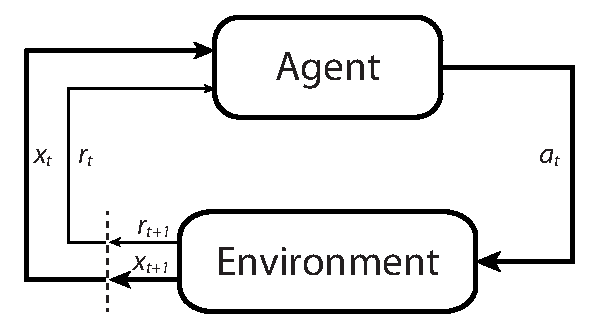
\includegraphics[width=.6\linewidth]{gfx/rl_loop.pdf}
\caption{The Reinforcement learning cycle}
\label{fig:rlloop}
\end{figure}

\subsection{Markov Decision Processes}

Markov Decision Process (MDP, \citet{bellman1957markovian}) is a classical formalization of sequential decision making, where actions influence not just immediate rewards, but also subsequent situations, or states, and through those future rewards. They are a mathematically idealized form of the reinforcement learning problem for which precise theoretical statements can be made.

The word Markov points to the fact that we assume that the state transitions of an MDP satisfy the Markov property \cite{???}. This means that the conditional probability distribution of future states of the process depends only upon the present state and not the whole history of events that preceded it.

\begin{definition}

MDP is a 5-tuple $\mathcal{M} = (\cX, \cA, R, P, \gamma)$, where 

$\cX$ is the finite state space

$\cA$ is the finite action space

$r(x, a)$ is a bounded deterministic\footnote{All the presented results are extendable to the case with random reward and with reward being a function of the transition $R(x, a, a')$. In fact, we use $R(x, a, a')$ in all our experiments. We avoid these extension to keep the n readable.} reward generated by being in state $x$ and selecting action $a$

$P(\cdot|x, a)$ is the transition probability distribution

$\gamma \in [0, 1)$ is a discount factor
\end{definition}

We will denote $x$ or $x_t$ as the states visited in time $t$ and $x'$ or $x_{t+1}$ states visited in time $t+1$. \unclear{weird? unify?}

\begin{definition}
A stationary (or Markovian) policy is a mapping from states to actions $\pi:\cX \to \cA$.
\end{definition}
\todo{deterministic cost doesn't go together with distributional :(}

%When solving MDPs with the usual discounted expected value criterion, it is common to limit the policy space to stationary policies, where the decision to take an action depends only on the current state. Unfortunately, when one considers other more general criteria, it is necessary to consider the whole action-state history that led up to the last state. This fact leads to the definition of a history-dependent policies.

\subsection{Return}

The ultimate goal of a reinforcement learning agent is to maximize some notion of reward, which is captured by the return. The two most commonly considered types of returns are the sum of rewards, or the mathematically convenient expected discounted reward. In this thesis we focus on the latter.


We define the return $Z^\pi(x)$ as a random variable representing the discounted reward along a trajectory generated by the MDP by following policy $\pi$, starting at state $x$:
\begin{equation}\label{eqn:return}
\begin{split}
&Z^\pi(x)=\sum_{t=0}^\infty \gamma^tR(x_t,a_t)\\
&x_t \sim p(\cdot|x_{t-1}, a_{t-1}), a_t \sim \pi, x_0 = x
\end{split}
\end{equation}

As a useful notation, we denote $Z^\pi(x, a)$ as the random variable representing the discounted reward along a trajectory generated by first selecting action $a$ and then following policy $\pi$.
\begin{equation}
\begin{split}
&Z^\pi(x, a)=\sum_{t=0}^\infty \gamma^tR(x_t,a_t)\\
&x_t \sim p(\cdot|x_{t-1}, a_{t-1}), a_t \sim \pi, x_0 = x, a_0 = a
\end{split}
\end{equation}

We will sometimes omit the superscript $\pi$ when the policy is clear from the context or is unimportant.

\subsection{Bellman equations}

The \textit{value function} $V^\pi : \cX\to\real$ of policy $\pi$ describes the expected return received from state $x \in \cX$ and acting according to $\pi$:
\begin{equation}
\begin{split}
V^\pi(x) = \expval{ Z^\pi(x)} =& \expect\left[\sum_{t=0}^\infty \gamma^tR(x_t,a_t) \right]\\
&x_0 = x, a_t \sim \pi
\end{split}
\end{equation}
The \textit{action-value} function $Q^\pi : \cX\times\cA\to\real$ of policy $\pi$ describes the expected return from taking action $a \in \cA$ from state $x \in \cX$, then acting according to $\pi$:
\begin{equation}
\begin{split}
Q^\pi(x, a) = \expval{Z^\pi(x, a)} =& \expect\left[ \sum_{t=0}^\infty \gamma^tR(x_t,a_t) \right]\\
&x_0 = x, a_0 = a, a_t \sim \pi
\end{split}
\end{equation}
Fundamental to reinforcement learning is the use of Bellman’s equation \citep{bellman1957markovian} to describe the value and action-value functions by a recursive relationship:
\begin{align}
&V^\pi(x) = R\left(x, \pi(x)\right) + \gamma \expect\limits_{p, \pi}[ V^\pi(x')]\\
&Q^\pi(x, a) = R(x, a) + \gamma \expect_{p, \pi}[ V^\pi(x')]
\end{align}
As stated before, we are typically interested in maximizing the expected return. The most common approach for doing so involves the optimality equation
\begin{equation}\label{eqn:q}
Q^*(x,a) = R(x,a) + \gamma \expect\nolimits_p \bsquare{\max_{a' \in \cA} Q^*(x', a')}
\end{equation}
This equation has a unique fixed point $Q^*$ -  the optimal value function, corresponding to the set of optimal policies $\Pi^*$ ($\pi^*$ is optimal if $\expect_{a \sim \pi^*} Q^*(x, a) = \max_a Q^*(x,a)$).
We view value functions as vectors in $\mathbb{R}^{\cX \times \cA}$, and the expected reward function as one such vector. In this context, the \emph{Bellman operator} $\cT^\pi$ and \emph{optimality operator} $\cT$ are
\begin{align}
\cT^\pi Q(x,a) &:= R(x, a) + \gamma \expect_{P, \pi} [Q(x',a')]\\
\cT Q(x,a) &:= R(x, a) + \gamma \expect_{P} \bsquare{\max_{a' \in \cA}Q(x', a')}\label{eqn:bellmanoptimalityoperator}
\end{align}
These operators are useful as they describe the expected behaviour of popular learning algorithms such as SARSA and Q-Learning \cite{sutton1998reinforcement}. In particular they are both contraction mappings (see below), and their repeated application to some initial $Q_0$ converges exponentially to $Q^\pi$ or $Q^*$, respectively \citep{bertsekas1995neuro}.

\subsection{Contraction}\label{sec:contraction}
An important concept used in convergence analysis of reinforcement learning algorithms is that of a contraction.
\begin{definition}
A \textbf{fixed point} of a mapping $T: S\to S$ of a set $S$ into itself is $s\in S$ which is mapped onto itself, that is $Ts=s$.

Let $S=(S,d)$ be a metric space ($d$ is a metric on $S$). A mapping $T$ is called a \textbf{contraction} on $S$ if there exists a positive real number $\gamma < 1$ such that for all $s, t \in S$ we have $d(Ts, Tt) \le \gamma d(s,t)$.
\end{definition}

\begin{theorem}[Banach Fixed Point Theorem, Contraction Theorem]
Consider a metric space $S=(S,d)$, where $S \neq \emptyset$. Suppose that $S$ is complete (every Cauchy sequence in $S$ converges) and let $T$ be a contraction on $S$. Then $T$ has precisely one fixed point.
\end{theorem}


The takeaway for reinforcement learning is, that if $\cT$ is a contraction, by recursively applying $V_{t+1}=\cT V_t$ (here the operator maps value function $V_t \in \real$ to a new $V_{t+1} \in \real$), we converge to the single fixed point of this operator. This is used in convergence proofs for various RL operators, usually in combination with the infinity norm.

See e.g. \citet{kreyszig1989introductory} for a complete treatment of all mentioned concepts.



%***********************************************************************************************************************************************************
%***********************************************************************************************************************************************************
%***********************************************************************************************************************************************************


\section{Distributional Reinforcement Learning}\label{sec:distrl}

In contrast to standard reinforcement learning, where we model the expected return, in distributional reinforcement learning \cite{many} we aim to model the full distribution of the return. This is advantageous in cases where we want to e.g. model parametric uncertainty \cite{...} or design risk-sensitive algorithms \citep{morimura2012parametric}\citep{morimura2010nonparametric}. \citet{bellemare2017distributional} also argue, that the distributional approach is beneficial even in the case when we optimize the expected value, as the distribution gives us more information which helps the now commonly used approximate algorithms (such as DQN \citep{mnih2015human}).

At the core of the distributional approach lies the recursive equation of the return distribution:
\begin{equation}
\begin{split}
&Z(x, a) \overset{D}{=} R(x, a) + \gamma Z(x', a')\\
&x' \sim p(\cdot|x, a), a \sim \pi, x_0 = x, a_0 = a
\end{split}
\end{equation}

where $\overset{D}{=}$ denotes that random variables on both sides of the equation share the same probability distribution.

In the \emph{policy evaluation} setting \citep{sutton1998reinforcement} we are interested in the value function $V^\pi$ associated with a given policy $\pi$. The analogue here is the value distribution $Z^\pi$. Note that $Z^\pi$ describes the intrinsic randomness of the agent's interactions with its environment, rather than some measure of uncertainty about the environment itself.
%

We define the transition operator $P^\pi : \mathcal{Z} \to \mathcal{Z}$
\begin{equation}
\begin{split}
&P^\pi Z(x, a) \overset{D}{=} Z(x', a')\\
&x' \sim p(\cdot|x, a), a' \sim \pi
\end{split}
\end{equation}
We define the distributional Bellman operator $\cT^\pi : \mathcal{Z} \to \mathcal{Z}$ as
\begin{equation}
\cT^\pi Z(x,a) \overset{D}{=} R(x,a) + \gamma P^\pi Z(x,a).
\end{equation}
Note that this is a distributional equation and the distributional bellman operator is therefore fundamentally different from the standard bellman operator.

\citet{bellemare2017distributional} have shown, that the distributional bellman operator $\cT^\pi$ is not a contraction in the commonly used KL divergence \cite{kullback1997information}, but is a contraction in the infinity Wasserstein metric which we describe bellow, as it will become useful as a tool for evaluating algorithms in the rest of the thesis. Another important fact is, that the bellman optimality operator $\cT : \mathcal{Z}\to\mathcal{Z}$
\begin{equation}
\cT Z = \cT^\pi Z \quad \text{for some } \pi \text{ in the set of greedy policies}
\end{equation}
is not a contraction in any metric. The distribution does not converge to a fixed point, but rather to a sequence of optimal (in terms of expected value) policies. We encourage the interested reader to explore these topics in the excellent papers by \citet{bellemare2017distributional} and \citet{dabney2017distributional}.

\subsection{The Wasserstein Metric}
\newcommand{\pnorm}[1]{\| #1 \|_p}

One of the tools for analysis of distributional approaches to reinforcement learning is the Wasserstein metric $d_p$ between cumulative distribution functions (see e.g. \citet{bickel1981some}). The metric has recently gained in popularity and was used e.g. in unsupervised learning \citep{arjovsky2017wasserstein,bellemare2017cramer}. Unlike the Kullback-Leibler divergence, which strictly measures change in probability, the Wasserstein metric reflects the underlying geometry between outcomes.

For $F$, $G$ two c.d.fs over the reals, it is defined as
\begin{equation*}
d_p(F, G) := \inf_{U, V} \pnorm{U - V},
\end{equation*}
where the infimum is taken over all pairs of random variables $(U, V)$ with respective cumulative distributions $F$ and $G$. The infimum is attained by the inverse c.d.f. transform of a random variable $\mathcal{U}$ uniformly distributed on $[0, 1]$:
\begin{equation*}
d_p(F, G) = \| F^{-1}(\mathcal{U}) - G^{-1}(\mathcal{U}) \|_p .
\end{equation*}
For $p < \infty$ this is more explicitly written as
\begin{equation}
d_p(F, G) = \left ( \int_0^1 \big | F^{-1}(u) - G^{-1}(u) \big |^p du \right )^{1/p} .
\end{equation}
meaning it is an integral over the difference in the quantile functions of the random variables. This will become important later, as the quantile function has a direct connection to the CVaR objective \eqnref{problem} explored in this thesis.


%***********************************************************************************************************************************************************
%***********************************************************************************************************************************************************
%***********************************************************************************************************************************************************


\section{Risk-Sensitivity}\label{sec:prelim:risk}

The standard reinforcement learning agent that maximizes the expected reward which we discussed in the previous chapter does not take risk into account. Indeed in a mathematical sense, the shape of the reward distribution is unimportant as wildly different distributions may have the same expectation. This unfortunately is not the case in the real world, where there exist catastrophic losses - an investment company may have a good strategy that yields profit in expectation, but if the strategy is too risky and the company's capital drops under zero this investment strategy is useless. This leads us to defining risk, which describes the potential of gaining or losing reward and is therefore more expressive than a simple expectation.

The finance literature differentiates between three risk-related types of behavior, namely \textit{risk-neutral}, \textit{risk-averse} and \textit{risk-seeking}. We offer the following example to illustrate the differences between mentioned behaviors: Imagine you are facing two options, either (a) you get \$1 or (b) you get \$5 with 90\% probability, but lose \$35 with 10\% probability. A risk-neutral agent wouldn't differentiate between the two choices, as the expected value of reward is the same. A risk-averse agent would prefer option (a), as there is a risk of high losses in option (b). Risk-seeking agent would pick (b). The difference between the risk-sensitive behaviors can be visualized as in \figref{risk}.

\begin{figure}
\center
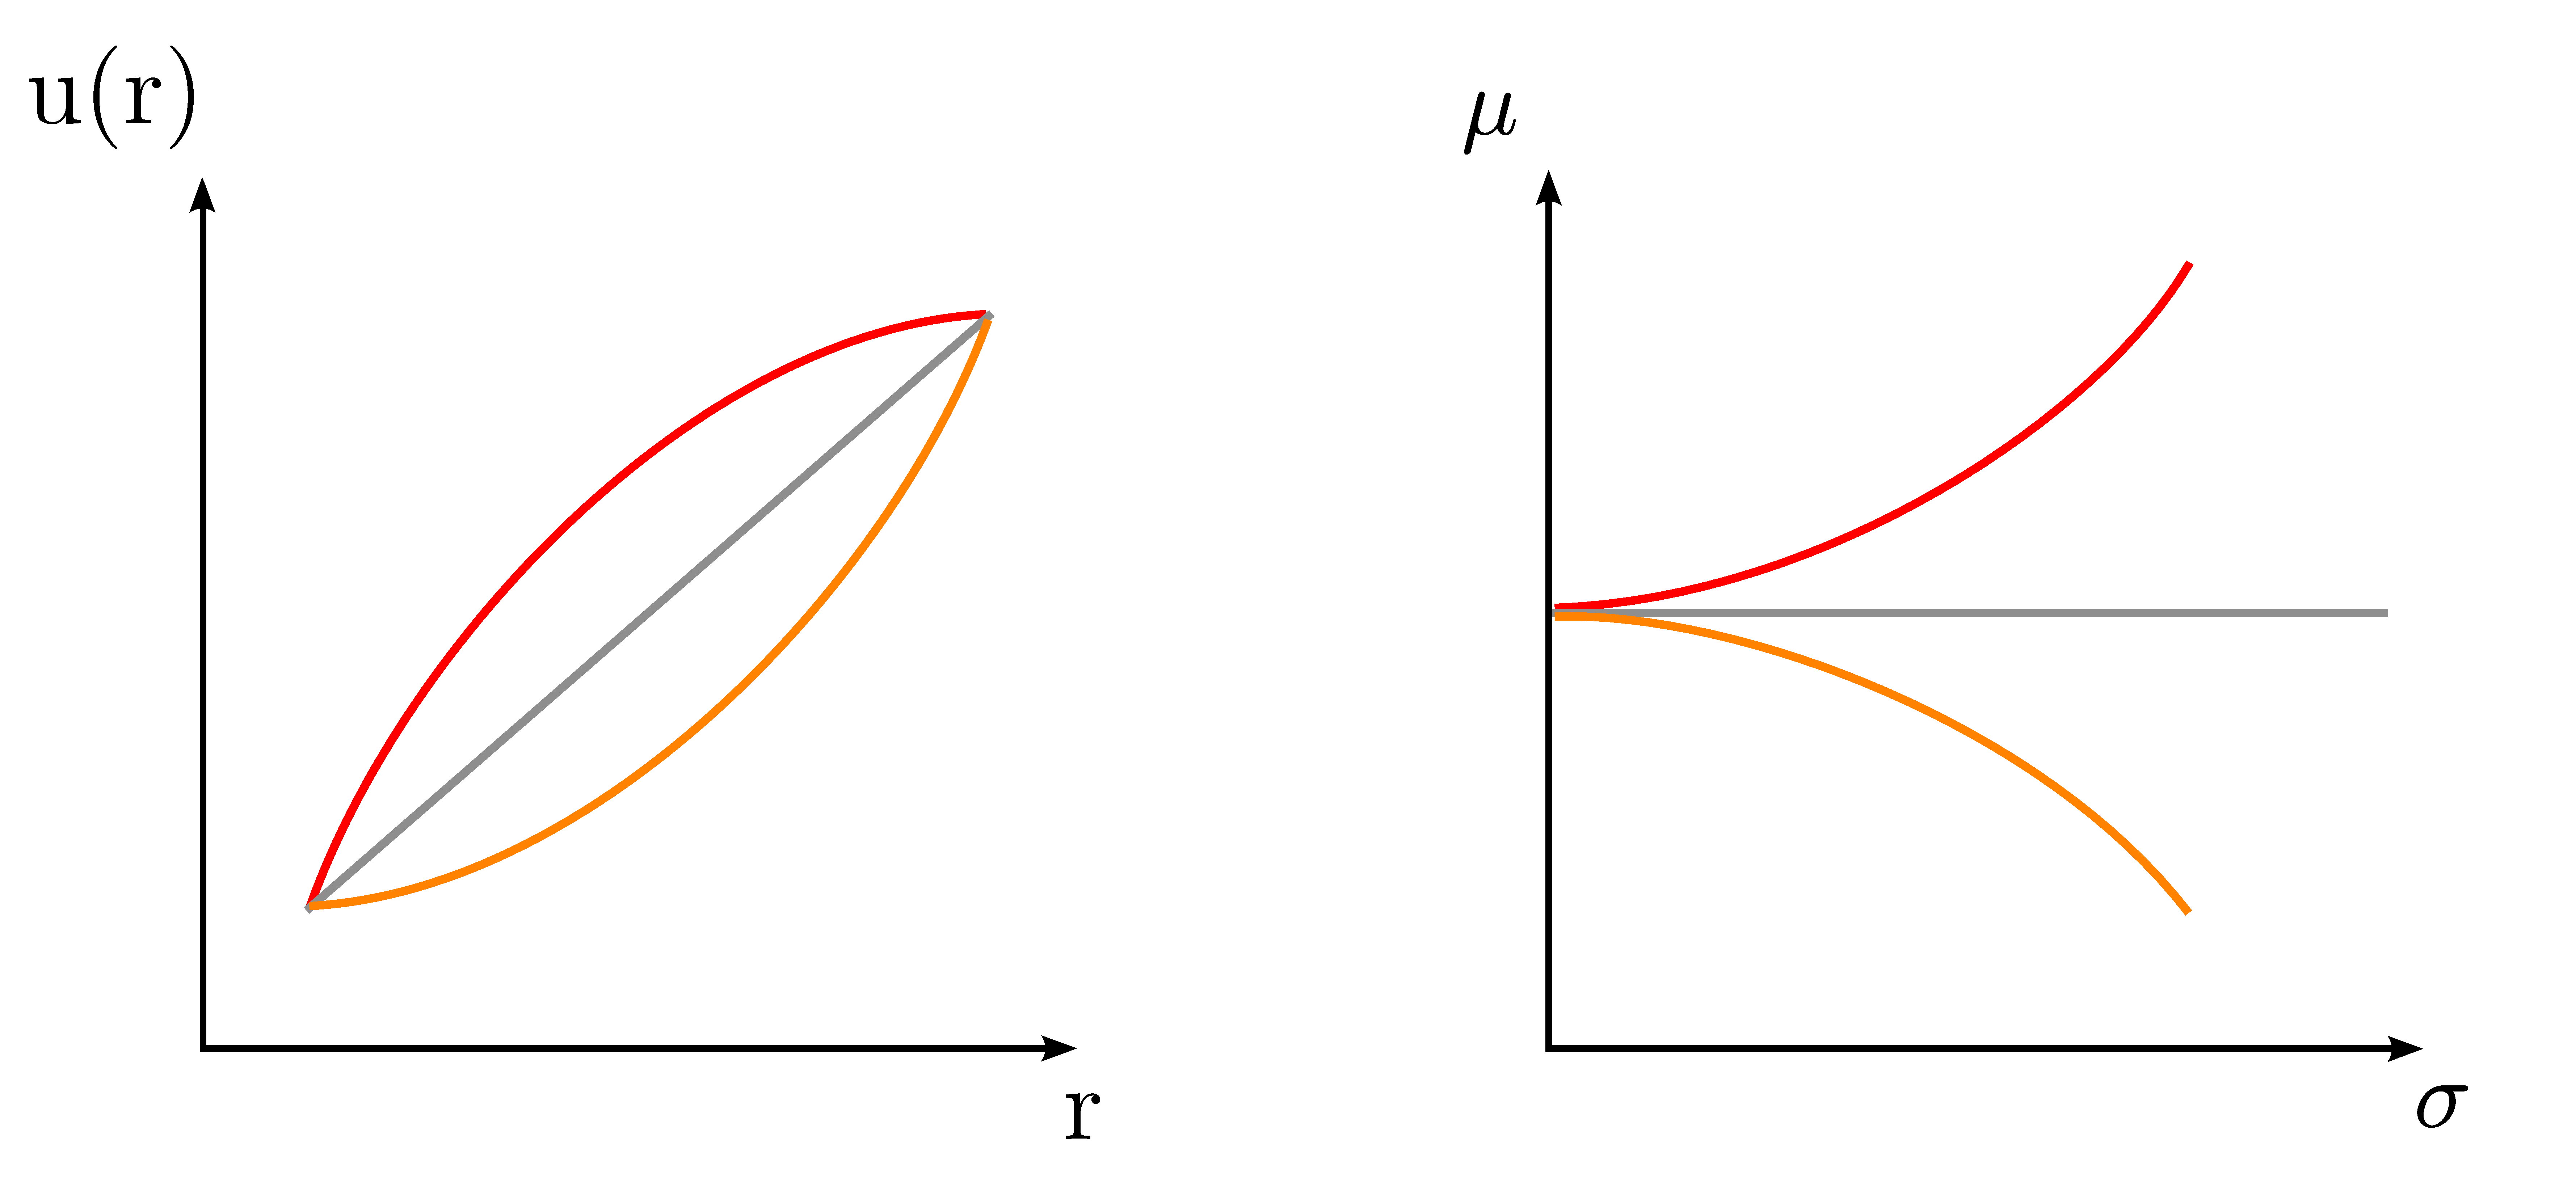
\includegraphics[width=0.8\linewidth]{gfx/risk.pdf}
\caption{Standard in economic literature, these figures depict the differences between risk-averse (red), risk-neutral (yellow) and risk-seeking (orange) behaviors.
\\
Left: A subjective utility $u(R)$, based on the reward, is concave for risk-averse behaviors. 
Right: Risk-averse utility contour lines in standard deviation-expected value space are upward sloped.
}
\label{fig:risk}
\end{figure}

The desired behavior for most critical applications is risk-averse and indeed it is the behavior of choice for financial institutions \citep{wipplinger2007philippe, basel2013fundamental}. ***It has also been suggested in the neuroscience literature, that humans use risk-averse behaviors when making decisions \citep{shen2014risk}.***

***As we stated in the introduction and will formally state in \secref{prelim:problem}, we are interested in reinforcement learning that maximizes a certain risk-averse objective. Below we formally describe the metrics used to measure risk which we then use to formulate the exact problem tackled in this thesis. ***


\subsection{Value-at-Risk}

Value-at-risk (VaR, see e.g. \citet{wipplinger2007philippe}) is one of the most popular tools used to estimate exposure to risk used risk management and financial control.

Let $Z$ be a random variable representing reward, with cumulative distribution function (c.d.f.) $F(z) = \mathbb{P}(Z \le z)$.
The Value-at-Risk  at confidence level $\alpha \in (0,1)$ is the $\alpha$-quantile of $Z$, i.e. 
\begin{equation}
\text{VaR}_\alpha(Z)=F^{-1}(\alpha)=\inf\left\lbrace z | \alpha \le F(z) \right\rbrace
\end{equation}

We will use the notation $\text{VaR}_\alpha(Z)$, $F^{-1}(\alpha)$ interchangeably, often explicitly denoting the random variable of inverse c.d.f. as $F^{-1}_Z(\alpha)$.
\\
\\
\textit{Note on notation}: In the risk-related literature, it is common to work with losses instead of rewards. The Value-at-Risk is then defined as the $1-\alpha$ quantile. The notation we use reflects the use of reward in reinforcement learning rather than losses and this sometimes leads to the need of reformulating some definitions or theorems. While these reformulations may differ in notation, they characterize the same underlying ideas.

\subsection{Conditional Value-at-Risk}

Conditional Value-at-Risk (CVaR, see \citet{rockafellar2000optimization,rockafellar2002conditional}), sometimes called Expected Shortfall (ES), Average Value-at-Risk (AVaR) or Tail Value-at-Risk (TVaR), is a risk measure that aims to fix inadequacies of measuring risk introduced by Value-at-Risk. Firstly, it has the desirable mathematical properties of monotonicity, translation invariance, positive homogeneity and subadditivity (see \citet{artzner1999coherent}), which makes CVaR computation much easier compared to VaR. It's properties were also recently identified as suitable for measuring risk in robotics \cite{majumdar2017should}. Another strong point of CVaR is that unlike VaR, it is able to distinguish between large and catastrophic losses. For these reasons, CVaR is starting to replace VaR as a standard measure for risk in financial applications \citep{basel2013fundamental} and beyond \cite{something}.

The Conditional Value-at-Risk (CVaR) at confidence level $\alpha \in (0,1)$ is defined as the expected reward of of outcomes worse than the $\alpha$-quantile ($\var_\alpha$):
\begin{equation}\label{eqn:cvardef}
\text{CVaR}_\alpha(Z) = \dfrac{1}{\alpha}\int_0^\alpha F^{-1}_Z(\beta) \text{d}\beta = \dfrac{1}{\alpha}\int_0^\alpha \text{VaR}_\beta(Z) \text{d}\beta
\end{equation}
\citet{rockafellar2000optimization} also showed that CVaR is equivalent to the solution of
\begin{equation}\label{eqn:cvarprimal}
\text{CVaR}_\alpha(Z)=
\max_s\left\lbrace \dfrac{1}{\alpha}\expect
\left[ (Z-s)^-\right] + s  \right\rbrace 
\end{equation}
where $(x)^- = \min(x, 0)$ represents the negative part of $x$ and in the optimal point $s^* = VaR_\alpha(Z)$
\begin{equation}
\text{CVaR}_\alpha(Z)= \dfrac{1}{\alpha}\expect \left[ (Z-VaR_\alpha(Z))^-\right] + VaR_\alpha(Z)
\end{equation}

The last definition we will need is the dual formulation of \eqnref{cvarprimal}
\begin{align}\label{eqn:cvardual}
&\text{CVaR}_\alpha(Z)= \min_{\xi \in \envelope}\expect\nolimits_\xi[Z]\\
&\envelope = \braces{\xi : \xi(\omega) \in \bsquare{0, \frac{1}{\alpha}}, \int_{\omega} \xi(\omega)\mathbb{P}(\omega) \text{d}\omega = 1}\label{eqn:envelope}
\end{align}


For a treatment of duality, see e.g. \citet{boyd2004convex}.

\begin{figure}
\center
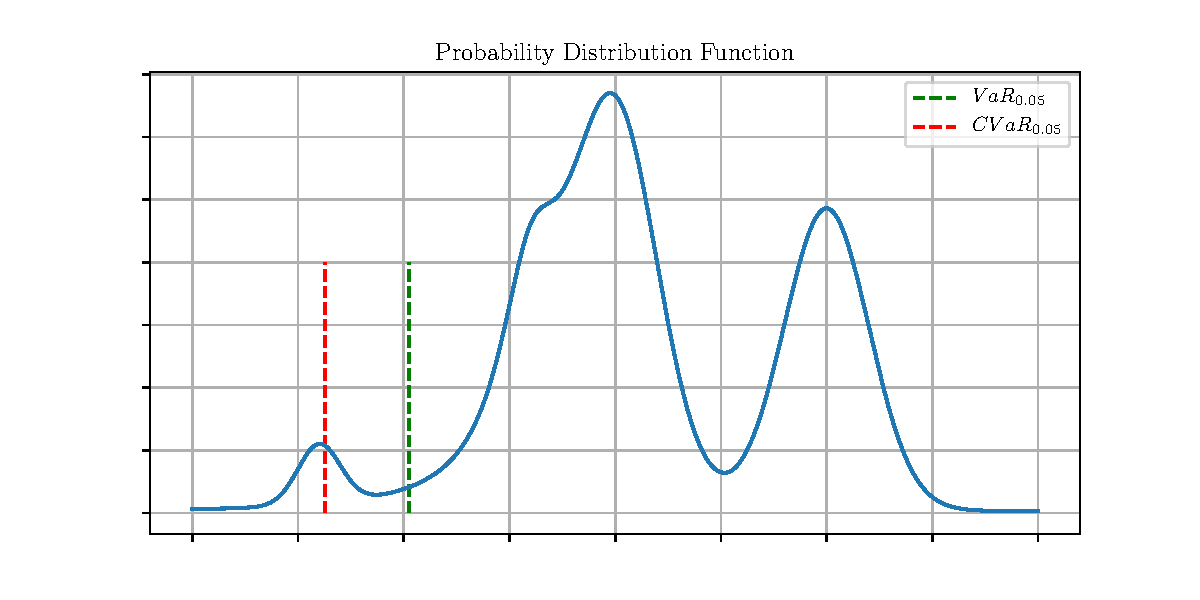
\includegraphics[width=\linewidth]{gfx/pdf.pdf}
\caption{Value-at-Risk and Conditional Value-at-Risk of a general probability distribution with the integral $\alpha=0.05$ marked in yellow. The main flaw of the VaR metric is clearly visible here, as we could shift the leftmost 'mode' of the distribution into minus infinity and the VaR would remain unchanged, while CVaR would change with the shift.}
\end{figure}




%*****************************************
%*****************************************
%*****************************************

\section{Problem Formulation}\label{sec:prelim:problem}

The problem tackled in this thesis considers reinforcement learning with optimization of the CVaR objective. Unlike the expected value criterion, it is insufficient to consider only stationary policies, and we must work with general history-dependent policies. We define them formally below.

\begin{definition}[History-Dependent Policies]
Let the space of admissible histories up to time $t$ be $H_t = H_{t-1} \times \cA \times \cX$ for $t \ge 1$, and $H_0 = \cX$. A generic element $h_t \in H_t$ is of the form $h_t = (x_0, a_0, ..., x_{t-1}, a_{t-1})$. Let $\Pi_{H,t}$ be the set of all history-dependent policies with the property that at each time $t$ the randomized control action is a function of $h_t$. In other words, 
$\Pi_{H,t} = \braces{\pi_0: H_0 \to \mathbb{P}(\cA), ..., \pi_t: H_t \to \mathbb{P}(\cA)}$. We also let $\Pi_H = \lim_{t\to\infty}\Pi_{H,t}$ be the set of all history-dependent policies.
\end{definition}

The risk-averse objective we wish to address for a given confidence level $\alpha$ is the following
\begin{equation}\label{eqn:problem}
\max_{\pi \in \Pi_H} \text{CVaR}_\alpha(Z^\pi(x_0))
\end{equation}
where $Z^\pi(x_0)$ coincides with definition \eqnref{return}.

In words, our goal is to find a general policy $\pi^*\in \Pi_H$, that maximizes conditional value-at-risk of the return, starting in state $x_0$. We emphasize the importance of the starting state since, unlike the expected value, the CVaR objective is not time-consistent.


\subsection{Time-consistency}\label{sec:time}

There exist several definitions of time-consistency \citep{pflug2016time, boda2006time}.
Informally, if the criterion is time-consistent, we can limit ourselves to the space of stationary policies, as the optimal policy is part of this space. On the other hand, non-stationary policies may be required to solve a time-inconsistent problem.

We provide the following example to show that the CVaR criterion is indeed time-inconsistent. On \figref{time-consistency} we can see an MDP with starting state $x_1$ with a single action $a_0$, followed by state $x_2$ where the agent can choose between actions $a_1, a_2$; states $x_3, x_4$ are terminal. We now compare three policies $\pi_1(x_1)=a_1, \pi_2(x_1)=a_2$ and a non-stationary policy $\pi_3$ that chooses $a_2$, unless the agent was lucky and received the reward 10 when transitioning from state $x_1$.
Let us examine the CVaR objective with $\alpha=0.19$ and $\gamma=1$ (or close to 1):
\begin{align*}
&\cvar_{0.19}(Z^{\pi_1}(x_1))=\frac{0.19 \cdot 0}{0.19} = 0\\
&\cvar_{0.19}(Z^{\pi_2}(x_1))=\frac{0.09\cdot (-10) + 0.01 \cdot 0 + 0.09 \cdot 10}{0.19}=0\\
&\cvar_{0.19}(Z^{\pi_3}(x_1))=\frac{0.09 \cdot (-10)+ 0.1 \cdot 10}{0.19} \cca 0.526
\end{align*}
By examining the results, we can see that the non-stationary policy $\pi_3$ is better than any stationary one, confirming CVaR as a time-inconsistent objective, explaining the need for a history-dependent policy in our problem definition \ref{eqn:problem}.

\begin{figure}
\center
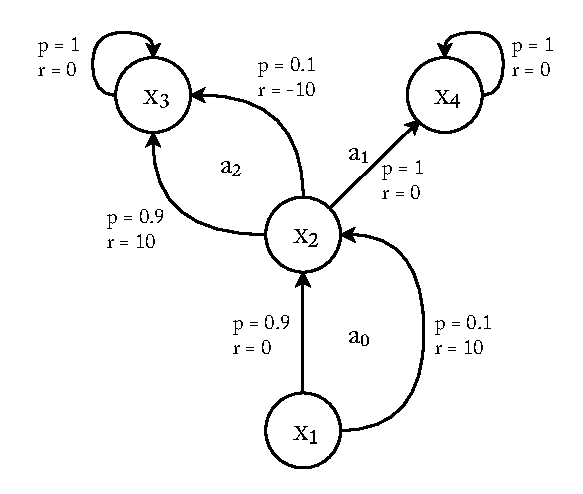
\includegraphics[width=0.6\linewidth]{gfx/time.pdf}
\caption{MDP showing time-inconsistency of the CVaR objective.}
\label{fig:time-consistency}
\end{figure}

\subsection{Robustness}

An important motivational point for the CVaR objective \eqnref{problem} is it's relationship with robustness. \citet{chow2015risk} have shown that optimizing the objective is equivalent to being robust to model perturbations. Thus, by minimizing CVaR, the decision maker also guarantees robustness to modeling errors. For completeness, we repeat the formulation of the equivalence relation below.

Let $(x_0, a_0, ..., x_T)$ be a trajectory in a finite-horizon MDP problem. The total probability of the trajectory is $P(x_0, a_0, ..., x_T)=P(x_0)P(x_1|x_0,a_0)\cdots P(x_T|x_{T-1}, a_{T-1})$. For each step $1\le t\le T$ consider a perturbed transition matrix $\hat{P} = P \circ \delta_t$ where $\delta_t \in \real^{\cX\times\cA\times\cX}$ and $\circ$ is the element-wise product under the condition that $\hat{P}$ is a stochastic matrix. Let $\Delta_t$ be the set of perturbation matrices that satisfy this condition and $\Delta = \Delta_1 \times \cdots \times \Delta_T$ be the set of all possible perturbations to the trajectory distribution.

We now impose a budget constraint on the perturbations as follows. For some budget $\eta \geq 1$, we consider the constraint
\begin{equation}\label{eqn:budget}
    \delta_1(x_1|x_0)\delta_2(x_2|x_1)\cdots \delta_T(x_T|x_{T-1}) \leq \eta
\end{equation}
Essentially, the product in \eqref{eqn:budget} states that \emph{the worst cannot happen at each time}. Instead, the perturbation budget has to be split (multiplicatively) along the trajectory. We note that \eqref{eqn:budget} is in fact a constraint on the perturbation matrices, and we denote by $\Delta_\eta \subset \Delta$ the set of perturbations that satisfy this constraint with budget $\eta$.
Then the following holds (Proposition 1 of \citep{chow2015risk})
\begin{equation}\label{eq:CVaR_is_robustness}
    \text{CVaR}_{\frac{1}{\eta}} \left(R_{0,T}(x_1,\dots,x_T)\right) = \inf_{(\delta_1,\dots,\delta_T)\in \Delta_{\eta}} \expect\nolimits_{\hat{P}}[R_{0,T}(x_1,\dots,x_T)],
\end{equation}
where $R_{0,T}(x_1,\dots,x_T)$ denotes the random variable representing the reward along the particular trajectory and $\expect\nolimits_{\hat{P}}[\cdot]$ denotes expectation with respect to a Markov chain with transitions $\hat{P}_t$.


%*****************************************
%*****************************************
%*****************************************



\section{Literature Survey}\label{sec:prelim:literature}

Risk-sensitive MDPs have been studied thoroughly in the past, with different risk-related objectives. Due to it's good computational properties, earlier efforts focused on exponential utility \citep{howard1972risk}, the max-min criterion \cite{minmax} or e.g. maximizing the mean with constrained variance \citep{sobel1982variance}. A comprehensive overview of the different objectives can be found in \citet{garcia2015comprehensive}, together with a unified look on the different methods used in safe reinforcement learning. Among CVaR-related objectives, some publications focus on optimizing the expected value with a CVaR constraint \citep{borkar2010risk, prashanth2014policy}.

Recently, for the reasons explained above, several authors have investigated the exact objective \eqnref{problem}. A considerable effort has gone towards policy-gradient \citep{sutton2000policy} and Actor-Critic \citep{konda2000actor} algorithms with the CVaR objective. \citet{tamar2015optimizing, chow2014algorithms} present useful ways of computing the CVaR gradients with parametric models and have shown the practicality and scalability of these approaches on interesting domains such as the well-known game of Tetris. An important setback of these methods is their limitation of the hypothesis space to the class of stationary policies, meaning they can only reach a $local$ minimum of our objective.
Similar policy gradient methods have also been investigated in the context of general coherent measures, a class of risk measures encapsulating many used measures including CVaR. Tamar et al. present a policy gradient algorithm \citep{tamar2017sequential} and a gradient-based Actor-Critic algorithm \citep{tamar2017sequential}. Again, these algorithms only converge in local extremes.

Some authors have also tried to sidestep the time-consistency issue of CVaR by either focusing on a time-consistent subclass of coherent measures \cite{???}, limiting the hypothesis space to time-consistent policies or reformulating the CVaR objective in a time-consistent way \cite{miller2017optimal}.

\citet{morimura2010nonparametric, morimura2012parametric} were among the first to utilize distributional reinforcement learning with both parametric and npnparametric models and used it to optimize CVaR, however they only used the naive approach discussed in \secref{time}.

\citet{bauerle2011markov} use a state space extensions and show that this new extended state space contains globally optimal policies. Unfortunately, because the state-space is continuous, the design of a solution algorithm is challenging.

The approach of \citet{chow2015risk} also uses a continuous augmented state-space but unlike \citet{bauerle2011markov}, this continuous state is shown to have bounded error when a particular linear discretization is used. The only flaw of this approach is the requirement of a linear program computation, which we address in the next chapter.

\todo{elaborate more on bauerle and chow (?)}

%Risk-sensitive MDPs have been studied for over four decades, with earlier efforts focusing on exponential utility \cite{Howard1972Risk}, mean-variance \cite{sobel_variance_1982}, and percentile risk criteria \cite{filar_percentile_1995} . Recently, for the reasons explained above, several authors have investigated CVaR MDPs \cite{rockafellar2000optimization}. Specifically, in \cite{borkar2014risk}, the authors propose a dynamic programming algorithm for finite-horizon risk-constrained MDPs where risk is measured according to CVaR. The algorithm is proven to asymptotically converge to an optimal risk-constrained policy. However, the algorithm involves computing  integrals over continuous variables (Algorithm 1 in \cite{borkar2014risk}) and, in general, its implementation appears particularly difficult. In \cite{bauerle2011markov}, the authors investigate the structure of CVaR optimal policies and show that a Markov policy is optimal on an augmented state space, where the additional (continuous) state variable is represented  by the running cost. In \cite{haskell2014convex}, the authors leverage such result to design an algorithm for CVaR MDPs that relies on discretizing occupation measures in the augmented-state MDP. This approach, however, involves solving a non-convex program via a sequence of linear-programming approximations, which can only shown to converge asymptotically. A different approach is taken by \cite{chow2014cvar} and \cite{tamar2015optimizing}, which consider a finite dimensional parameterization of control policies, and show that a CVaR MDP can be optimized to a \emph{local} optimum using stochastic gradient descent (policy gradient). A recent result by Pflug and Pichler \cite{pflug2012time} showed that CVaR MDPs admit a dynamic programming formulation by using a state-augmentation procedure different from the one in \cite{bauerle2011markov}. The augmented state  is also continuous, making the design of a solution algorithm challenging. 

%\subsection{Safe Reinforcement Learning}
%
%\citep{garcia2015comprehensive}
%\citep{bauerle2011markov}
%
%
%
%
%\subsection{Reinforcement Learning with CVaR-related criteria}
%
%*** Policy gradient literature ignores the time consistency-issue, leading to locally optimal policies show that they can be worse than EXP ***.
%\citep{tamar2015policy}
%\citep{tamar2015optimizing}
%\citep{chow2014algorithms}



%\part{Reinforcement Learning with CVaR}\label{pt:core}

%************************************************
\chapter{Value Iteration with CVaR}\label{ch:vi}
%************************************************

Value iteration is a standard algorithm for maximizing expected discounted reward used in reinforcement learning. In this chapter we extend the results of \citet{chow2015risk}, who have recently proposed an approximate value iteration algorithm for CVaR MDPs. 

The original algorithm requires the computation of a linear program in each step of the value iteration procedure. Utilizing a connection between the used $\alpha \cvar_\alpha$ function and the quantile function, we sidestep the need for this computation and propose a linear-time version of the algorithm, making CVaR value iteration feasible for much larger MDPs. 

After reminding the reader of the standard value iteration algorithm, we present the original algorithm in \secref{vi:cvar}. The improved algorithm is presented in  \secref{vi:linear}, followed by section \secref{vi:experiments}, where we test the algorithm on selected environments.

%*****************************************

\section{Value Iteration}

Value iteration \citep{sutton1998reinforcement} is a well-known algorithm for computing the optimal (action-)value function and hereby finding the optimal policy. Let us remind ourselves of the Bellman optimality operator $\cT$ \eqnref{bellmanoptimalityoperator}:
\begin{equation*}
\cT Q(x,a) := \expval{ R(x, a)} + \gamma \expect\nolimits_{P} \bsquare{\max_{a' \in \cA}Q(x', a')}
\end{equation*}
or rewritten for the value function $V$
\begin{equation}
\cT V(x) := \max_a\braces{\expval{ R(x, a)} + \gamma \expect\nolimits_{P} \bsquare{V(x')}}
\end{equation}
As stated before, $\cT$ is a contraction (\secref{contraction}). This means that by repeatedly applying the operator we eventually converge to the optimal point, since we converge and the definition holds in this point. This leads to the formulation of the \textit{Value Iteration} algorithm. The only difference between theory and practice is the introduction of a small parameter $\epsilon$ that allows us to check the converge and end the algorithm when we reach a certain precision, as the contraction converges only in the limit.

See \algref{vi}.


\begin{algorithm}
\caption{Value Iteration}
\label{alg:vi}
\begin{algorithmic}
    \STATE Initialize $V$ arbitrarily (e.g. $V(x)=0$ for all $x \in \cX$)
    
	\REPEAT
	
	\STATE $v = V(x)$
	\STATE $\Delta = 0$
	
	\FOR{each $x \in \cX$}
	\STATE $V(x) = \max_a\braces{r(x, a) + \gamma\sum_{s'}p(s'|x, a)V(x')}$
	\STATE $\Delta = \max\braces{\Delta, |v-V(x)|}$
	\ENDFOR
	
	\UNTIL{ $\Delta < \epsilon$ }
	
	\STATE Output a deterministic policy $\pi \approx \pi^*$:
   	\STATE $\quad\quad \pi(x) = \argmax_a\braces{r(x, a) + \gamma\sum_{s'}p(s'|x, a)V(x')}$
\end{algorithmic}
\end{algorithm}


\section{CVaR Value Iteration}\label{sec:vi:cvar}

\citet{chow2015risk} present a dynamic programming formulation for the CVaR MDP problem \eqnref{problem}. As CVaR is a time-inconsistent measure, their method requires an extension of the state space. A Value Iteration type algorithm is then applied on this extended space and \citet{chow2015risk} proved it's convergence. 

We repeat their key ideas and results bellow, as they form a basis for our contributions presented in later sections. The results are presented with our notation introduced in \chref{prelim}, which differs slightly from the paper, but the core ideas remain the same.

\subsection{Bellman Equation for CVaR}

The results of \citet{chow2015risk} heavily rely on the CVaR decomposition theorem (Lemma 22, \citep{pflug2016time}):
%
\begin{equation}\label{eqn:cvardecomp}
CVaR_\alpha\bround{Z^\pi(x)} = \min_{\xi \in \envelope} \sum_{x'} p(x'| x, \pi(x))\xi(x') CVaR_{\xi(x')\alpha}\bround{Z^\pi(x')}
\end{equation}
%
where the risk envelope $\envelope$ coincides with the dual definition of CVaR \eqnref{envelope}.
The theorem states that we can compute the $CVaR_\alpha\bround{Z^\pi(x, a)}$ as the minimal (or worst-case) weighted combination of $CVaR_\alpha\bround{Z^\pi(x')}$ under a probability distribution perturbed by $\xi(x')$.

Note that the decomposition requires only the representation of CVaR at different confidence levels and not the whole distribution at each level, which we might be tempted to think because of the time-inconsistency issue.

\citet{chow2015risk} extend the decomposition theorem by defining the \emph{CVaR value function} $V(x, y)$ with an augmented state-space $\mathcal{X}\times\mathcal{Y}$ where $\mathcal{Y}=(0,1]$ is an additional continuous state that represents the different confidence levels.
%
\begin{equation}
V(x, y)=\max_{\pi \in \Pi_H} \cvar_{y}\bround{Z^\pi(x)}
\end{equation}
%
Similar to standard dynamic programming, it is convenient to work with with operators defined on the space of value functions. This leads to the following definition of the CVaR Bellman operator $\mathbf{T}:\mathcal{X}\times\mathcal{Y}\to\mathcal{X}\times\mathcal{Y}$:
%
\begin{equation}
\mathbf{T}V(x, y) = \max_a \bsquare{ R(x, a) + \gamma \min_{\xi \in \envelope} \sum_{x'} p(x'| x, a)\xi(x') V\bround{x', y\xi(x')}}
\end{equation}
%
or in our simplified notation:
%
\begin{equation}\label{eqn:tcvar}
\mathbf{T} CVaR_y(Z(x))=\max_a \bsquare{R(x, a) + \gamma CVaR_{y}(Z(x, a))}
\end{equation}
%
\citet{chow2015risk} further showed (Lemma 3) that the operator $\mathbf{T}$ is a contraction and also preserves the convexity of $y CVaR_t$. The optimization problem \eqnref{cvardecomp} is a convex one and therefore has a unique solution. Additionally, the fixed point of this contraction is the optimal $V^*(x, y) = \max_{\pi \in \Pi} CVaR_y (Z^\pi(x, y))$ (\citep{chow2015risk}, Theorem 4).
 
The value-function $V^*$ can then be used to extract the optimal policy $\pi^*$ of the original problem \eqnref{problem}, using the following theorem.

\begin{theorem}[Optimal Policies, Theorem 5 in \citep{chow2015risk}]\label{thm:optimalpolicy}
Let $\pi_H^*=\{\mu_0,\mu_1,\ldots\}\in\Pi_H$ be a history-dependent policy recursively defined as:
\begin{equation}\label{eqn:policy_construct}
\mu_k(h_k) = u^*(x_k, y_k),\,\,\forall k\geq 0,
\end{equation}
with initial conditions $x_0$ and $y_0=\alpha$, and state transitions
\begin{equation}\label{eqn:opt_state}
x_k\sim P(\cdot\mid x_{k-1},u^*(x_{k-1},y_{k-1})),\quad y_k = y_{k-1}\xi_{x_{k-1},y_{k-1},u^*}^*(x_k), \forall k\geq 1,
\end{equation}
where the stationary Markovian policy $u^*(x,y)$ and risk factor $\xi_{x,y,u^*}^*(\cdot)$ are solution to the  max-min optimization problem in the CVaR Bellman operator $\mathbf T[V^*](x,y)$.
Then, $\pi^*_H$ is an optimal policy for problem \eqnref{problem} with initial state $x_0$ and CVaR confidence level $\alpha$.
\end{theorem}


Naive value iteration with operator $\mathbf{T}$ is unfortunately unusable in practice, as the state space is continuous in $y$. The solution proposed in \cite{chow2015risk} is then to represent the convex $y\cvar_y$ as a piecewise linear function. 

\subsection{Value Iteration with Linear Interpolation}

Given a set of $N(x)$ interpolation points $\mathbf{Y}(x) = \braces{y_1, \dots, y_{N(x)}}$, we can interpolate the $yV(x,y)$ function on these points, i.e.
%
\begin{equation*}
\interpI_{x}[V](y)=y_iV(x,y_{i})+\frac{y_{i+1}V(x,y_{i+1})-y_iV(x,y_{i})}{y_{i+1}-y_i}(y-y_i),
\end{equation*}
%
where $y_i = \max \left\{y'\in \mathbf{Y}(x) : y' \leq y\right\}$
The interpolated Bellman operator $\mathbf{T}_\interpI$ is then also a contraction and has a bounded error (\citep{chow2015risk}, Theorem 7). 
\todo{bounded -> linear in $\theta$}
%
\begin{equation}\label{eqn:linearbellman}
\mathbf{T}_\interpI V(x, y) = \max_a \bsquare{ R(x, a) + \gamma \min_{\xi \in \envelope} \sum_{x'} p(x'| x, a)\dfrac{\interpI_{x'} [V](y\xi(x'))}{y}}
\end{equation}
%
The full value iteration procedure is presented in \algref{cvarlinear}. 

This algorithm can be used to find an approximate global optimum in any MDP. There is however the issue of computational complexity. As the algorithm stands, the straightforward approach is to solve each iteration of \eqnref{linearbellman} as a linear program, since the problem is convex and piecewise linear, but this is not practical, as the LP computation can be demanding and is therefore not suitable for large state-spaces.

\unclear{maybe formulate the LP exactly?}

In the next section we aim to find a different way of computing the optimization problem.

\begin{algorithm}[h]
\caption{\texttt{CVaR Value Iteration with Linear Interpolation}}
\label{alg:cvarlinear}
1: \textbf{Given:}
\begin{itemize}
%\item An interpolation error bound $\epsilon>0$ for small CVaR thresholds.
\item $N(x)$ interpolation points $\mathbf{Y}(x)  = \left\{y_1,\dots,y_{N(x)}\right\} \in [0,1]^{N(x)}$ for every $x\in \mathcal X$ with $y_i<y_{i+1}$, $y_1=0$ and $y_{N(x)}=1$.
%, $y_2 = \min_{x',a}\{ P(x'|x,a):P(x'|x,a)\neq 0\}$
%\item An interpolation function $\interpI_{x}[V](y;\interpY(x))$ for $yV(x,y)$ for any arbitrary value function $V$.
\item Initial value function $V_0(x,y)$ that satisfies:
\begin{enumerate}
\item $yV_0(x,y)$ is convex in $y$ for all $x$
\item $yV_0(x,y)$ is continuous in $y$ for all $x$
\end{enumerate}
 %where $V_0(x,y)=0$ at $y<0$.
\end{itemize}
2: Repeat until convergence:
\begin{itemize}
%\item Update the smallest non-zero grid $y_2$ in $\interpY(x)$ by choosing it to satisfy $\max_{x\in\mathcal X, y\in \mathbf I_2(x)}|V_0(x,y_2)-V_0(x,y)|\leq\epsilon$, where the interpolation based Bellman operator $ \bellint$ is given by
%  \[
%\hspace{-0.5in}  \bellint[V](x,y) =
% \min_{a\in\mathcal A}\left[C(x,a)+\gamma\max_{\xi\in \U_{\text{CVaR}}(y, P(\cdot|x,a))}\sum_{x'\in\mathcal X}\frac{\interpI_{x'}[V](y\xi(x');\interpY(x'))}{y}P(x'|x,a)\right].
%   \]
\item For each $x \in \mathcal X$ and each $y_i\in \mathbf{Y}(x)$, update the value function estimate as follows:
  \begin{equation*}
   V_{k+1}(x,y_i)= \mathbf{T}_\interpI[V_k](x,y_i),
  \end{equation*}
  \end{itemize}
3: Set the converged value iteration estimate as $\widehat{V}^*(x,y_i)$, for any $x\in\mathcal X$, and $ y_i\in\mathbf{Y}(x)$.
\end{algorithm}


%*****************************************

\section{Efficient computation using quantile representation}\label{sec:vi:linear}

We present our original contributions in this section. We first describe a connection between the $y\cvar_y$ function and the quantile function of the underlying distribution. We then use this connection to formulate a faster computation of the value iteration step, resulting in the first linear-time algorithm for solving CVaR MDPs with bounded error.

\begin{lemma}\label{thm:varcvarconnection}
Any discrete distribution has a piecewise linear and convex $y\cvar_y$ function. Similarly, any piecewise linear convex function can be seen as representing a certain discrete distribution.
\\
Particularly, the integral of the quantile function is the $y\cvar_y$ function
\begin{equation}\label{eqn:varcvarintegration}
y\cvar_y(Z) = \int_0^y VaR_\beta(Z) \dt \beta
\end{equation}
and the derivative of the $y\cvar_y$ function is the quantile function
\begin{equation}\label{eqn:varcvarderivation}
\dfrac{\partial}{\partial y} y \cvar_y(Z) = VaR_y(Z)
\end{equation}
\end{lemma}

\begin{proof}
The fact that discrete distributions have has already been shown by \citet{rockafellar2000optimization}.
\\
According to definition \eqnref{cvardef} we have
\begin{equation*}
y\cvar_y(Z) = y\dfrac{1}{y}\int_0^y VaR_\beta(Z) \dt \beta = \int_0^y VaR_\beta(Z) \dt \beta
\end{equation*}
by taking the $y$ derivative, we have
\begin{equation*}
\dfrac{\partial}{\partial y} y \cvar_y(Z) = \dfrac{\partial}{\partial y} \int_0^y VaR_\beta(Z) d\beta = VaR_y(Z)
\end{equation*}
\end{proof}

You can get some intuition from \figref{cvarvisual}, where the integral-derivation relationship is clearly visible.

According to Lemma \ref{thm:varcvarconnection}, we can reconstruct the $y\cvar_y$ from the underlying distribution and vice-versa. We utilize the fact that the conversion is linear in the number of probability atoms to formulate a fast way of computing the $\mathbf{T}_\interpI$ operator.

\begin{figure}
\center
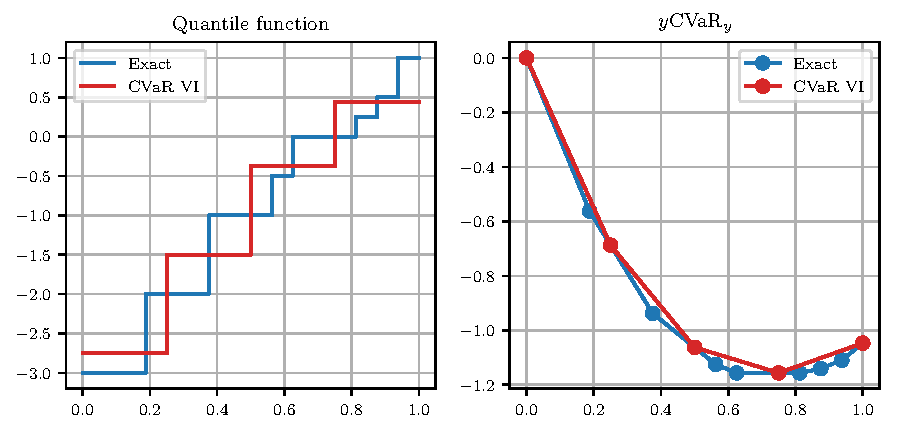
\includegraphics[width=\linewidth]{gfx/cvar_visualized.pdf}
\caption{Comparison of a discrete distribution and it's approximation according to the CVaR linear interpolation operator.}
\label{fig:cvarvisual}
\end{figure}

\subsection{CVaR Computation via Quantile Representation}

We propose the following procedure: instead of using linear programming for the CVaR computation, we use the underlying distributions represented by the $\alpha CVaR_\alpha$ function to compute CVaR.

The computation of CVaR of a discrete probability mixture is a linear-time process as we show bellow. The general steps of the computation are as follows

\begin{enumerate}
\item transform $y \cvar_y$ of each possible state transition to a discrete probability distribution function using \eqnref{varcvarderivation}
\item combine these to to a distribution representing the full state-action distribution
\item compute $y \cvar_y$ for all atoms using \eqnref{varcvarintegration}
\end{enumerate}
See \figref{cvarcomputation} for a visualization of the procedure.

\begin{figure}
\center
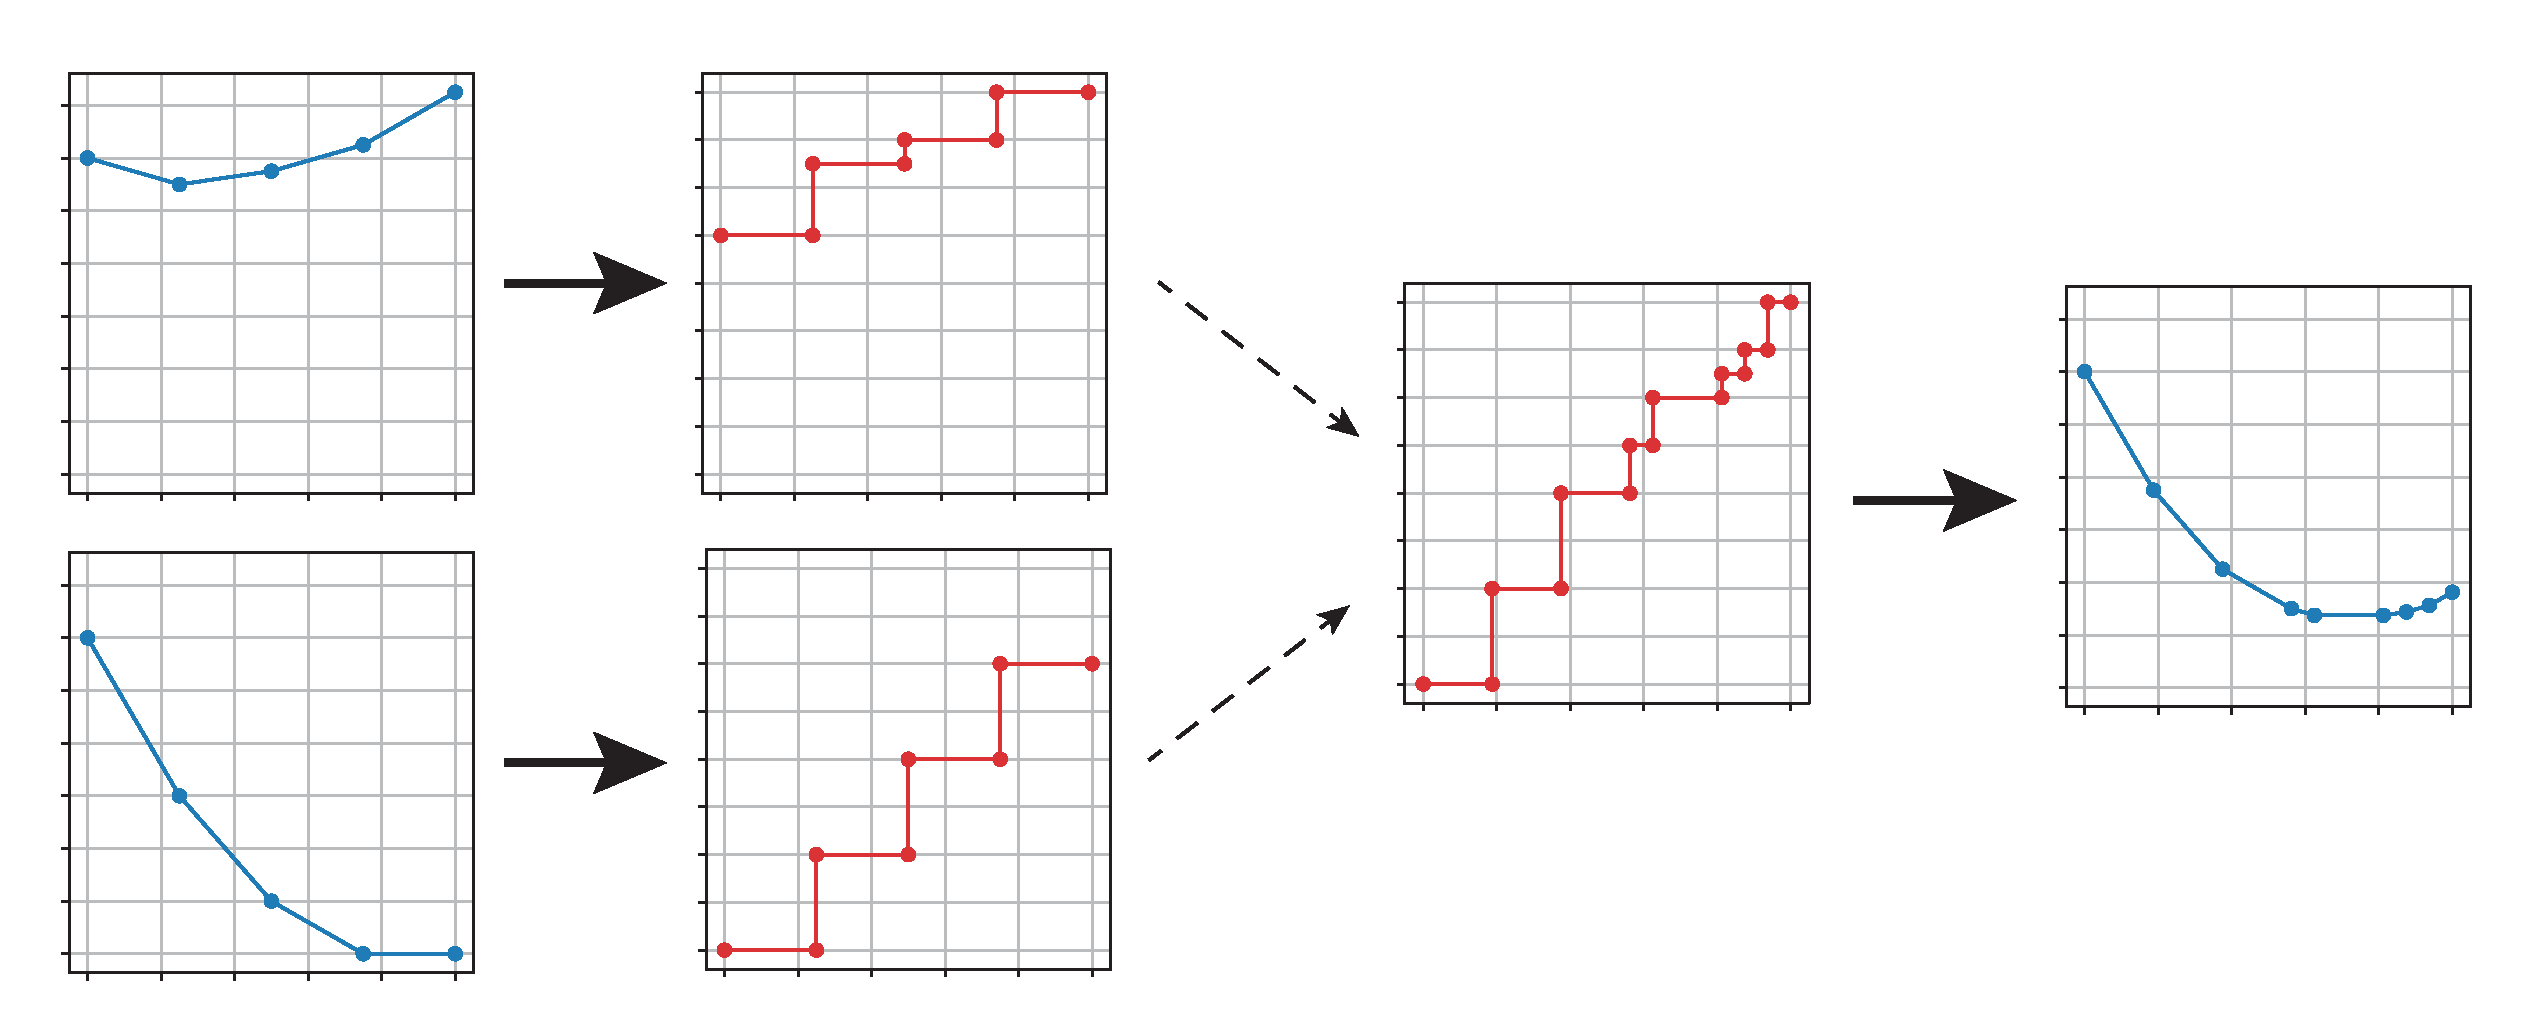
\includegraphics[width=\linewidth]{gfx/cvar_vi_conversion.pdf}
\caption{Visualization of the CVaR computation for a single state and action with two transition states. Thick arrows represent the conversion between $\ycvary$ and the quantile function.}
\label{fig:cvarcomputation}
\end{figure}

\todo{show the linearity}
\unclear{show an example computation?}

\unclear{proof necessary? also, maybe it is already in the $\xi$ proof}


%\begin{algorithm}
%\caption{CVaR computation}
%
%\begin{multicols}{2}
%
%\begin{algorithmic}
%    \STATE \textbf{input} $\alpha, x_t, \pi_\text{old}, \gamma$
%    \WHILE{$x_t$ is not terminal}
%    	\STATE $a = \text{arg}\max_a CVaR_\alpha(Z(x_t, a))$
%		\STATE $s = VaR_\alpha(Z(x_t, a))$
%		\columnbreak
%
%    	\STATE $x_t, r_t = \text{envTransition}(x_t, a)$
%    	\STATE $\alpha = F_{Z(x_t, \pi_\text{old}(x_t))}\left(\dfrac{s - r}{\gamma}\right) $ \textcolor{gray}{\# $VaR_\alpha(Z(x_t, \pi_\text{old}(x_t))) == \dfrac{s - r}{\gamma}$}
%   	\ENDWHILE
%\end{algorithmic}
%\end{multicols}
%\end{algorithm}
%
%\begin{minipage}[t]{0.5\linewidth}
%  \vspace{0pt}  
%  \begin{algorithm}[H]
%    \caption{Algo 1}
%    line 1\;
%    line 2\;
%  \end{algorithm}
%\end{minipage}%
%\begin{minipage}[t]{5cm}
%  \vspace{0pt}
%  \begin{algorithm}[H]
%    \caption{Algo 1}
%    line 1\;
%  \end{algorithm}
%\end{minipage}

\subsection{$\xi$-computation}

Similarly to \thmref{optimalpolicy}, we need a way to compute the $y_{k+1}=y_{k}\xi^*(x_k)$ to extract the optimal policy. Again, we can skip the LP computation by using the following intuition: $y_{k+1}$ is the portion of $Z(x_{k+1})$ that is present in $\cvar_{y_k}(Z(x_k))$. In the continuous case, it is the probability in $Z(x_{k+1})$ before the $\var_{y_k}(Z(x_k))$ as we show bellow.

\todo{proof for discrete distributions}

\begin{theorem}
Solution to minimization problem \eqnref{cvardecomp} can be computed without optimization by setting
\begin{equation}\label{eqn:xi-claim}
\xi ( x' ) = \dfrac{F_{x'}(F^{-1}_x(\alpha))}{\alpha} 
\end{equation}
\end{theorem}

\begin{proof}
For simplification, we work only with two states: $x'$ the actual sampled state and $\bar{x}'$ representing the other states. The equation then simplifies to

\begin{equation}\label{eqn:cvardecomp2}
\begin{split}
CVaR_\alpha(x, a)&=\min_{\xi} \, p\xi CVaR_{\xi\alpha}(x') + (1-p)\dfrac{1-p\xi}{1-p}CVaR_{\frac{1-p\xi}{1-p}\alpha}(\bar{x}')\\
&=\min_{\xi} \, p\xi CVaR_{\xi\alpha}(x') + (1-p\xi)CVaR_{\frac{1-p\xi}{1-p}\alpha}(\bar{x}')\\
\end{split}
\end{equation}

To find the min we first find the first derivative\footnote{
We used the following identities:
\begin{equation*}
\dfrac{\partial CVaR_{\alpha\xi}}{\partial \xi} = \frac{1}{\xi}VaR_{\xi\alpha}-\frac{1}{\xi}CVaR_{\xi\alpha}\quad\quad\quad
\dfrac{\partial CVaR_{\frac{1-p\xi}{1-p}\alpha}}{\partial\xi} = \frac{p}{1-p\xi}CVaR_{\frac{1-p\xi}{1-p}\alpha}	-	\frac{p}{1-p\xi}VaR_{\frac{1-p\xi}{1-p}\alpha}
\end{equation*}
} w.r.t. $\xi$

\begin{equation}
\begin{split}
\dfrac{\partial CVaR_\alpha}{\partial \xi} &= pCVaR_{\xi\alpha} + p\xi \dfrac{\partial CVaR_{\alpha\xi}}{\partial \xi} - pCVaR_{\frac{1-p\xi}{1-p}\alpha} + (1 - p\xi)\dfrac{\partial CVaR_{\frac{1-p\xi}{1-p}\alpha}}{\partial\xi}\\
&= pCVaR_{\xi\alpha} + p\xi\left[	\frac{1}{\xi}VaR_{\xi\alpha}-\frac{1}{\xi}CVaR_{\xi\alpha}	\right] - pCVaR_{\frac{1-p\xi}{1-p}\alpha} \\&\hspace*{5cm} + (1-p\xi)\left[	\frac{p}{1-p\xi}CVaR_{\frac{1-p\xi}{1-p}\alpha}	-	\frac{p}{1-p\xi}VaR_{\frac{1-p\xi}{1-p}\alpha}\right]\\
&= pCVaR_{\xi\alpha} + pVaR_{\xi\alpha} - pCVaR_{\xi\alpha} - pCVaR_{\xi\alpha} - pCVaR_{\frac{1-p\xi}{1-p}\alpha} \\&\hspace*{5cm} + CVaR_{\frac{1-p\xi}{1-p}\alpha} - pVaR_{\frac{1-p\xi}{1-p}\alpha}\\
&= pVaR_{\xi\alpha} - pVaR_{\frac{1-p\xi}{1-p}\alpha}
\end{split}
\end{equation}

By setting the derivative to 0 (to find the min), we get
\begin{equation}\label{eqn:varvar}
VaR_{\xi\alpha}(x')= VaR_{\frac{1-p\xi}{1-p}\alpha}(\bar{x}')
\end{equation}

By inserting claim \eqnref{xi-claim} into \eqnref{varvar} we get the symmetrical claim
\begin{equation}
\dfrac{1-p\xi}{1-p} = \xi(\bar{x}') = \dfrac{F_{\bar{x}'}(F^{-1}_x(\alpha))}{\alpha}
\end{equation}

We rewrite \eqnref{cvardecomp2} as (assuming $\xi$ is the minimum point)

\begin{equation}
\begin{split}
\frac{1}{\alpha} \int_0^\alpha F^{-1}_{x}(t)dt &= p\xi \frac{1}{\xi\alpha} \int_0^{\xi\alpha} F^{-1}_{x'}(t)dt + (1-p\xi)\frac{1-p}{(1-p\xi)\alpha} \int_0^{\frac{1-p\xi}{1-p}\alpha} F^{-1}_{\bar{x}'}(t)\\
&=p \frac{1}{\alpha} \int_0^{\xi\alpha} F^{-1}_{x'}(t)dt + (1-p)\frac{1}{\alpha} \int_0^{\frac{1-p\xi}{1-p}\alpha} F^{-1}_{\bar{x}'}(t)
\end{split}
\end{equation}

This must also hold if we multiply both sides by $\alpha$
\begin{equation}
\int_0^\alpha F^{-1}_{x}(t)dt = p\int_0^{\xi\alpha} F^{-1}_{x'}(t)dt + (1-p)\int_0^{\frac{1-p\xi}{1-p}\alpha} F^{-1}_{\bar{x}'}(t)
\end{equation}
And we take derivations w.r.t. $\alpha$ of both sides
\begin{equation}
F^{-1}_{x}(\alpha) = p\xi F^{-1}_{x'}(\xi\alpha) + (1-p\xi) F^{-1}_{\bar{x}'}(\frac{1-p\xi}{1-p}\alpha)
\end{equation}


By inserting \eqnref{xi-claim} we get
\begin{equation}
\begin{split}
 p\xi F_{x'}^{-1}(\xi\alpha) + (1-p)\xi_2 F_{\bar{x}'}^{-1}\left(\xi_2\alpha\right) &= p\xi F_{x'}^{-1}(F_{x'}(F^{-1}_x(\alpha))) + (1-p\xi) F_{\bar{x}'}^{-1}\left(F_{\bar{x}'}(F^{-1}_x(\alpha))\right)\\
 &= p\xi F_x^{-1}(\alpha) + (1-p\xi)F_x^{-1}(\alpha) = F_x^{-1}(\alpha)
\end{split}
\end{equation}

We've shown that the proposed solution \eqnref{xi-claim} satisfies the minimization constraint \eqnref{varvar} (= is a minimal point) and satisfies the dual decomposition \eqnref{cvardecomp}. (This has been shown only in the differentiated form )

\end{proof}


%*****************************************



\section{Experiments}\label{sec:vi:experiments}

\todo{$|\mathcal{X}|\sim 1M$ tabular environment}

\todo{get matlab code from tamar}

\subsection{Cliffworld}

\section{Summary}


%*****************************************
%*****************************************
%*****************************************
%*****************************************
%*****************************************





%************************************************
\chapter{Q-learning with CVaR}\label{ch:qlearning}
%************************************************

While value iteration is a useful algorithm, it only works when we have complete knowledge of the environment - including the probability transitions $p(x'|x,a)$. This is often not the case in practice and we have to rely on different methods, based on direct interaction with the environment. One such algorithm is the well-known Q-learning which we explore in this chapter.

We first remind the reader of Q-learning basics in \secref{qlearning} and introduce CVaR estimation in \secref{cvarestimation}. These concepts are combined together with CVaR value iteration and in \secref{qcvar} we propose the new CVaR Q-learning algorithm. We treat the optimal policy separately in \secref{qpolicy}.

The algorithm is then experimentally verified on suitable environments in \secref{qexperiments}.

%***********************************************************************************************************************************************************
%***********************************************************************************************************************************************************
%***********************************************************************************************************************************************************
\section{Q-learning}\label{sec:qlearning}

Q-learning (\citet{watkins1992q}) is an important off-policy Temporal Difference control algorithm, that works by repeatedly updating the $Q$ value estimate according to the sampled rewards and states using a moving exponential average.
\begin{equation}
\begin{split}
&Q_{t+1}(x, a) = (1-\beta_t)Q_{t}(x, a) + \beta_t\bsquare{r + \gamma \max_{a'} Q_t(x', a')}\\
&x' \sim p(\cdot|x, a)
\end{split}
\end{equation}
Here $Q$ is an estimate of the optimal action-value function \eqnref{q} and $\beta_t$ is the learning rate at time $t$. The expression $r + \gamma \max_{a'} Q_t(x', a')$ is called a \textit{target} and is sometimes denoted as $\cT Q$. The idea of the algorithm is to bring the value function closer to the target, which is more 'informed' than the original value since it has information about the reward and next state, which came directly from the sampled transition. The optimal value of $Q(x, a)$ is then the expected target, which we reach in the limit.

The order of the visited states is unimportant, as long as all reachable states are updated infinitely often and the learning rate meets a standard condition used in stochastic approximation.
\begin{equation}\label{eqn:beta}
\sum_{t=0}^\infty \beta_t = \infty  \quad \sum_{t=0}^\infty \beta_t^2 < \infty\\
\end{equation}
See \citet{jaakkola1994convergence} for details.

While the algorithm would converge if we were using a completely random policy, in practice we often try to speed up the convergence by using a smarter, yet still random policy as seen in \algref{qlearning}.


\begin{algorithm}
\caption{Q-learning}
\begin{algorithmic}\label{alg:qlearning}
    \STATE Initialize $Q(x, a)$ for all $x \in \cX, a \in \cA$ arbitrarily, and $Q(x_\text{terminal}, \cdot) = 0$
    
	\FOR{each episode}
	
	\STATE $x = x_0$
	
	\WHILE{$x$ is not terminal}
	\STATE Choose $a$ using a policy derived from $Q$ (e.g. $\varepsilon$-greedy)
	\STATE Take action $a$, observe $r, x'$
	\STATE $Q(x, a) = (1-\beta_t)Q(x, a) + \beta_t\bsquare{r + \gamma \max_{a'} Q(x', a')}$
	\STATE $x = x'$	
	\ENDWHILE
	
	\ENDFOR
\end{algorithmic}
\end{algorithm}


\section{CVaR estimation}\label{sec:cvarestimation}

Before formulating a CVaR version of Q-learning, we must first talk about simply \emph{estimating} CVaR, as it is not as straightforward as the estimation of expected value.

Let us remind ourselves of the primal definition of CVaR \eqnref{cvarprimal}:
\begin{equation*}
\cvar_\alpha(Z)=
\max_s\left\lbrace \dfrac{1}{\alpha}\expect
\left[ (Z-s)^-\right] + s  \right\rbrace 
\end{equation*}
If we knew the exact $s^*=\var_\alpha$, we could estimate the CVaR as a simple expectation of the $\dfrac{1}{\alpha}(Z-s^*)^-+s^*$ function. As we do not know this value in advance, a common approach is to first approximate $\var_\alpha$ from data, then use this estimate to compute its $\cvar_\alpha$. This is usually done with a full data vector, requiring the whole data history to be saved in memory.

When dealing with reinforcement learning, we would like to store our current estimate as a scalar instead. This requires finding a recursive expression whose expectation is the CVaR value. Fortunately, similar methods have been thoroughly investigated in the stochastic approximation literature by \citet{robbins1951stochastic}.

The RM theorem has also been applied directly to CVaR estimation by \citet{bardou2009recursive}, who used it to formulate a recursive importance sampling procedure useful for estimating CVaR of long-tailed distributions.

First let us describe the method for one step estimation, meaning we sample values (or rewards in our case) $r$ from some distribution and our goal is to estimate CVaR at a given confidence level $\alpha$. The procedure requires us to maintain two separate estimates $V$ and $C$, being our VaR and CVaR estimates respectively.
\begin{align}
V_{t+1} &= V_{t} + \beta_t \bsquare{1-\dfrac{1}{\alpha}\indicator_{(V_t \ge r)}}\label{eqn:varestimate}\\
C_{t+1} &= (1-\beta_t)C_t + \beta_t \bsquare{V_t + \dfrac{1}{\alpha}(r-V_t)^-}\label{eqn:cvarestimate}
\end{align}
An observant reader may recognize a standard equation for quantile estimation in equation \eqnref{varestimate} (see e.g. \citet{koenker2001quantile} for more information on quantile estimation/regression). The expectation of the update $\expect\bsquare{1-\dfrac{1}{\alpha}\indicator_{(V_t \ge r)}}$ is the inverse gradient of the CVaR primal definition, so we are in fact performing a Stochastic Gradient Descent on the primal.

Equation \eqnref{cvarestimate} is also quite intuitive, representing the moving exponential average of the primal CVaR definition \eqnref{cvarprimal}. The estimations are proven to converge, given the usual requirements on the learning rate \eqnref{beta} \citep{bardou2009recursive}.

%***********************************************************************************************************************************************************
%***********************************************************************************************************************************************************
%***********************************************************************************************************************************************************

\section{CVaR Q-learning}\label{sec:qcvar}

We now extend the previously established CVaR Value Iteration and combine it with the recursive CVaR estimation techniques to formulate a new algorithm we call CVaR Q-learning.

\subsection{Temporal Difference update}
We first define two separate values for each state, action, and atom $V, C: \cX\times\cA\times\cY\to\real$ where $C(x, a, y)$ represents $\cvar_y(Z(x, a))$ of the distribution, similar to the definition \eqnref{cdef}. $V(x, a, y)$ represents the $\var_y$ estimate, i.e. the estimate of the $y-$quantile of a distribution recovered from $\cvar_y$ by Lemma \ref{thm:varcvarconnection}.

A key to any temporal difference algorithm is its update rule. The CVaR TD update rule extends the improved value iteration procedure and we present the full rule for uniform atoms in \algref{cvartd}. 

Let us now go through the algorithm step by step. We first construct a new CVaR (line \ref{alg:cvartd:1}), representing $\cvar_y(Z(x'))$, by greedily selecting actions that yield the highest CVaR for each atom. This is in contrast with both standard Q-learning and Quantile Regression Q-learning (\secref{dqn:qrdqn}) where we select a single action for the whole distribution.
This step is implicit in the CVaR value iteration procedure since we are not working with action-value functions. 

The new values $C(x', \bigcdot)$ are then transformed to the underlying distribution (line \ref{alg:cvartd:2}) $\mathbf{d}$ and used to create the target $\cT \mathbf{d} = r + \gamma \mathbf{d}$. A natural Monte Carlo approach would be then to generate samples from this target distribution and use these to update our estimates $V, C$.

Since we know the target distributions exactly, we do not have to actually sample; instead we use the quantile values proportionally to their probabilities (in the uniform case, this means exactly once) and apply the respective VaR and CVaR update rules (lines \ref{alg:cvartd:4}, \ref{alg:cvartd:5}).


\begin{algorithm}
\caption{CVaR TD update}
\begin{algorithmic}[1]\label{alg:cvartd}

    \STATE \textbf{input:} $x, a, x', r$
    
    \FOR{each $i$ }
	\STATE $C(x', y_i) = \max_{a'} C(x', a', y_i)$ \label{alg:cvartd:1}
	\ENDFOR
	
	\STATE $\mathbf{d}= \text{extractDistribution}\bround{C(x', \bigcdot), \mathbf{y}}$ \comment{See \algref{cvarvi}}\label{alg:cvartd:2}

	\FOR{each $i, j$}
	\STATE $V(x, a, y_i) = V(x, a, y_i) + \beta \bsquare{1 - \frac{1}{y_i}\indicator_{(V(x, a, y_i) \ge r+\gamma d_j)}}$  \label{alg:cvartd:4}
	\STATE $C(x, a, y_i) = (1-\beta)C(x, a, y_i) + \beta\bsquare{V(x, a, y_i) + \frac{1}{y_i}\bround{r+\gamma d_j - V(x, a, y_i)}^-}$\label{alg:cvartd:5}
	\ENDFOR
\end{algorithmic}
\end{algorithm}

If the atoms aren't uniformly spaced (log-spaced atoms are motivated by the error bounds of CVaR Value Iteration), we have to perform basic importance sampling when updating the estimates . In contrast with the uniform version, we iterate only over the atoms and perform a single update for the whole target by taking an expectation over the target distribution. This is done by replacing lines \ref{alg:cvartd:4}, \ref{alg:cvartd:5} with
\begin{equation}
\begin{split}
V(x, a, y_i) &= V(x, a, y_i) + \beta \expect_j\bsquare{1 - \frac{1}{y_i}\indicator_{(V(x, a, y_i) \ge r+\gamma d_j)}}\\
C(x, a, y_i) &= (1-\beta)C(x, a, y_i) + \beta\expect_j\bsquare{V(x, a, y_i) + \frac{1}{y_i}\bround{r+\gamma d_j - V(x, a, y_i)}^-}
\end{split}
\end{equation}
The explicit computation of the expectation term for VaR would then look like
\begin{equation*}
\expect_j\bsquare{1 - \frac{1}{y_i}\indicator_{(V(x, a, y_i) \ge r+\gamma d_j)}} = \sum_j p_j\bsquare{1 - \frac{1}{y_i}\indicator_{(V(x, a, y_i) \ge r+\gamma d_j)}}
\end{equation*}
where $p_j = y_{j}-y_{j-1}$ represents the probability of $d_j$. The CVaR update expectation is computed analogically.
%$$ \expect_j\bsquare{V(x, a, y_i) + \frac{1}{y_i}\bround{r+\gamma d_j - V(x, a, y_i)}^-} = \sum_j p_j\bsquare{V(x, a, y_i) + \frac{1}{y_i}\bround{r+\gamma d_j - V(x, a, y_i)}^-}$$

This is a valid approach since sample mean is equal to the mean of the original distribution. In this case we are performing the updates on batches of samples and the final expected value remains unchanged.
\begin{equation*}
\mathbb{E}[f(Z)] = \sum_i p_i \mathbb{E}[f(Z_i)]
\end{equation*}
The above equation holds for any function $f$ if $Z$ is a mixture of $Z_i$, so it also holds for the VaR update $1 - \frac{1}{y_i}\indicator_{(V(x, a, y_i) \ge r+\gamma d_j)}$ where the learned distribution is a mixture of the different target distributions.

We conclude the same for the CVaR update, since the expectation remains unchanged. 

We are in fact using more informed updates - similar to the difference between pure and batch Stochastic Gradient Descent.
%
%\begin{algorithm}
%\caption{CVaR TD update - general case}
%\begin{algorithmic}\label{alg:cvartdg}
%
%    \STATE \textbf{input:} $x, a, x', r$
%    
%    \FOR{each $y_i$ }
%	\STATE $C(x', y_i) = \max_{a'} C(x', a', y_i)$ \label{alg:cvartdg:1}
%	\ENDFOR
%	
%	\STATE $\mathbf{d}= \text{extractDistribution}\bround{C(x', \bigcdot), \mathbf{y}}$ \label{alg:cvartdg:2} \comment{See \algref{cvarvi}}\label{alg:cvartd:2}
%
%	\FOR{each $i$}
%	\STATE $V(x, a, y_i) = V(x, a, y_i) + \beta \expect_j\bsquare{1 - \frac{1}{y_i}\indicator_{(V(x, a, y_i) \ge r+\gamma d_j)}}$  \label{alg:cvartd:4}
%	\STATE $C(x, a, y_i) = (1-\beta)C(x, a, y_i) + \beta\expect_j\bsquare{V(x, a, y_i) + \frac{1}{y_i}\bround{r+\gamma d_j - V(x, a, y_i)}^-}$\label{alg:cvartdg:5}
%	\ENDFOR
%\end{algorithmic}
%\end{algorithm}

\subsection{Note on convergence}
We do not prove the convergence of the CVaR Q-learning algorithm in this thesis as it would require significant work regarding convergence of the recursive CVaR estimation procedures. The update rules (\ref{eqn:varestimate}, \ref{eqn:cvarestimate})  have been only shown to converge if the underlying distributions are continuous \citep{bardou2009recursive}, which is not the case in our setting.


In the last section of this chapter, we show at least empirical convergence of the CVaR Q-learning algorithm.

%***********************************************************************************************************************************************************
%***********************************************************************************************************************************************************
%***********************************************************************************************************************************************************


\section{Optimal Policy}\label{sec:qpolicy}

Recall that in CVaR Value Iteration we can extract the optimal policy by recursively setting $y_{t+1}=y_t \xi^*_{x_{t+1}}$. This process is not straightforwardly extendable to our sample-based version of CVaR Value Iteration, since we would have to have access to all possible transition states and probabilities in order to compute $\xi^*$.

Instead, we turn to the primal formulation of CVaR in what we call VaR-based policy improvement algorithm. We first introduce the VaR-based policy improvement in the context of distributional RL and prove its validity. The policy improvement procedure is then used as a consistent heuristic for extracting the optimal policy from converged CVaR Value Iteration.


\subsection{VaR-based Policy Improvement}

Let us now assume that we have successfully converged with distributional value iteration and have available the return distributions of some stationary policy for each state and action. Our next goal is to find a policy improvement algorithm that will monotonically increase the $\cvar_\alpha$ criterion for selected $\alpha$.

Recall the primal definition of CVaR \eqnref{cvarprimal}
\begin{equation*}
\text{CVaR}_\alpha(Z)=
\max_s\left\lbrace \dfrac{1}{\alpha}\expect
\left[ (Z-s)^-\right] + s  \right\rbrace 
\end{equation*}
Our goal \eqnref{problem} can then be rewritten as
\begin{equation*}
\max_\pi \cvar_\alpha(Z^\pi) = \max_\pi \max_s \dfrac{1}{\alpha}\mathbb{E}
\left[ (Z^\pi-s)^-\right] + s
\end{equation*}
As mentioned earlier, the primal solution is equivalent to $\var_\alpha(Z)$
\begin{equation*}
\cvar_\alpha(Z)=
\max_s\left\lbrace \dfrac{1}{\alpha}\mathbb{E}
\left[ (Z-s)^-\right] + s  \right\rbrace =\dfrac{1}{\alpha}\mathbb{E}
\left[ (Z - \text{VaR}_\alpha(Z))^-\right] + \text{VaR}_\alpha(Z) 
\end{equation*}

The main idea of VaR-based policy improvement is the following: If we knew the value $s^*$ in advance, we could simplify the problem to maximize only
\begin{equation}\label{eqn:varbasedgoal}
\max_\pi \cvar_\alpha(Z^\pi) = \max_\pi \dfrac{1}{\alpha}\mathbb{E}
\left[ (Z^\pi-s^*)^-\right] + s^*
\end{equation}
Given that we have access to the return distributions, we can improve the policy by simply choosing an action that maximizes $\cvar_\alpha$ in the first state $a_0 = \text{arg}\max_\pi\text{CVaR}_\alpha(Z^\pi(x_0))$, setting $s^* = \var_\alpha(Z(x_0, a_0))$ and focus on maximization of the simpler criterion.

This can be seen as coordinate ascent with the following phases:
\begin{enumerate}
\item Maximize $\frac{1}{\alpha}\mathbb{E}\left[ (Z^\pi(x_0)-s)^-\right] + s$ w.r.t. $s$ while keeping $\pi$ fixed. This is equivalent to computing CVaR according to the primal.
\item Maximize $\frac{1}{\alpha}\mathbb{E}\left[ (Z^\pi(x_0)-s)^-\right] + s$ w.r.t. $\pi$ while keeping $s$ fixed. This is the policy improvement step.
\item Recompute $\cvar_\alpha (Z^{\pi^*})$ where $\pi^*$ is the new policy.
\end{enumerate}
Since our goal is to optimize the criterion of the distribution starting at $x_0$, we need to change the value $s$ while traversing the MDP (where we have only access to $Z(x_t)$). We do this by recursively updating the $s$ we maximize by setting $s_{t+1} = \dfrac{s_t - r}{\gamma}$. See \algref{varbasedpi} for the full algorithm which we justify in the following theorem.

\begin{algorithm}
\caption{VaR-based policy improvement}
\label{alg:varbasedpi}
\begin{algorithmic}
    \STATE $a = \text{arg}\max_a \cvar_\alpha(Z(x_0, a))$
    \STATE $s = \var_\alpha(Z(x_0, a))$
    \STATE Take action $a$, observe $x, r$
    \WHILE{$x$ is not terminal}
    	\STATE $s = \dfrac{s-r}{\gamma}$
    	\STATE $a = \text{arg}\max_a \mathbb{E}\left[(Z(x, a)-s)^- \right]$
    	\STATE Take action $a$, observe $x, r$
   	\ENDWHILE
\end{algorithmic}
\end{algorithm}

\begin{theorem}
Let $\pi$ be a stationary policy, $\alpha \in (0, 1]$. 
By following policy $\pi^*$ from algorithm \ref{alg:varbasedpi}, we improve $CVaR_\alpha(Z)$ in expectation:
$$CVaR_\alpha(Z^\pi) \le CVaR_\alpha(Z^{\pi^*})$$
%
%Let policy $\pi'$ constructed the following way: Set $\pi'(x_0) = \text{arg}\max_\pi\cvar_\alpha(Z^\pi(x_0))$ and $s = \var_\alpha(Z^\pi(x_0, \pi'(x_0)))$. Each following step set $s = $
%

\end{theorem}

\begin{proof}

Let $s^*$ be a solution to $\max_s \dfrac{1}{\alpha}\mathbb{E}\left[ (Z^\pi(x_0)-s)^-\right] + s$. Then by optimizing $\dfrac{1}{\alpha}\mathbb{E}
\left[ (Z^\pi-s^*)^-\right]$ over $\pi$, we monotonously improve the optimization criterion $CVaR_\alpha(Z(x_0))$.
\begin{align*}
\cvar_\alpha(Z^{\pi}) &= \max_{s}\dfrac{1}{\alpha}\mathbb{E}\left[ (Z^{\pi}-s)^-\right] + s &&= \dfrac{1}{\alpha}\mathbb{E}\left[ (Z^{\pi}-s^*)^-\right] + s^* \\
&\le \max_{\pi'}\dfrac{1}{\alpha}\mathbb{E} \left[ (Z^{\pi'}-s^*)^-\right] + s^* &&= \dfrac{1}{\alpha}\mathbb{E}\left[ (Z^{\pi^*}-s^*)^-\right] + s^*\\
 &\le \max_{s'}\dfrac{1}{\alpha}\mathbb{E}\left[ (Z^{\pi^*}-s')^-\right] + s' &&= CVaR_\alpha(Z^{\pi^*})
\end{align*}

When optimizing w.r.t. $\pi$ we can ignore the scaling term $\frac{1}{\alpha}$ and a constant term $s^*$ without affecting the optimal argument. We can therefore focus on optimization of $\mathbb{E}\left[ (Z^\pi(x_0)-s^*)^-\right]$.
\begin{equation}
\begin{split}
\mathbb{E}\left[(Z_t-s)^-\right] &= \mathbb{E}\left[(Z_t-s)\mathbb{1}(Z_t\le s)\right] = \mathbb{E}\left[(r_t + \gamma Z_{t+1}-s)\mathbb{1}(Z_{t+1}\le \dfrac{s - r_t}{\gamma})\right]\\
&= \sum_{x_{t+1}, r_t} P(x_{t+1}, r_t \given x_t, a)\mathbb{E}\left[(r_t + \gamma Z(x_{t+1})-s)\mathbb{1}(Z(x_{t+1})\le \dfrac{s - r_t}{\gamma})\right]\\
&= \sum_{x_{t+1}, r_t} P(x_{t+1}, r_t \given x_t, a)\mathbb{E}\left[\gamma\left(Z(x_{t+1})-\dfrac{s-r_t}{\gamma}\right)\mathbb{1}(Z(x_{t+1})\le \dfrac{s - r_t}{\gamma})\right]\\
&= \gamma\sum_{x_{t+1}, r_t} P(x_{t+1}, r_t \given x_t, a)\mathbb{E}\left[\left(Z(x_{t+1})-\dfrac{s-r_t}{\gamma}\right)\mathbb{1}(Z(x_{t+1})\le \dfrac{s - r_t}{\gamma})\right]\\
&= \gamma\sum_{x_{t+1}, r_t} P(x_{t+1}, r_t \given x_t, a)\mathbb{E}\left[\left(Z(x_{t+1}) - \dfrac{s - r_t}{\gamma}\right)^-\right]
\end{split}
\end{equation}
where we used the definition of return $Z_t = R_t + \gamma Z_{t+1}$ and the fact that probability mixture expectations can be computed as $\mathbb{E}[f(Z)] = \sum_i p_i \mathbb{E}[f(Z_i)]$ for any function $f$.

Now let's say we sampled reward $r_t$ and state $x_{t+1}$, we are still trying to find a policy $\pi^*$ that maximizes 
\begin{equation}\label{eqn:sampled x_t+1}
\begin{split}
\pi^* &=\text{arg}\max_\pi \mathbb{E}\left[(Z(x_t)-s)^-\right | x_{t+1}, r_t]\\
&= \text{arg}\max_\pi \mathbb{E}\left[\left(Z(x_{t+1}) - \dfrac{s - r_t}{\gamma}\right)^-\right]
\end{split}
\end{equation}

Where we ignored the unsampled states, since these are not a function of $x_{t+1}$, and the multiplicative constant $\gamma$ that will not affect the maximum argument.

At the starting state, we set $s=s^*$. At each following state we select an action according to equation \eqnref{sampled x_t+1}. By induction we maximize the criterion \eqnref{varbasedgoal} in each step.
\end{proof}

Note that while the resulting policy is nonstationary, we do not need an extended state-space to follow this policy. It is only necessary to remember our previous value of $s$.

The ideas presented here were partially explored by \citet{bauerle2011markov} although not to this extent. See Remark 3.9 in \citep{bauerle2011markov} for details.

\subsection{CVaR Q-learning extension}
We would now like to use the policy improvement algorithm in order to extract the optimal policy from CVaR Q-learning. This would mean optimizing $\mathbb{E}\left[(Z_t-s)^-\right]$ in each step. A problem we encounter here is that we have access only to the discretized distributions and we cannot extract the values between selected atoms.

As a solution to this, we propose an approximate heuristic that uses linear interpolation to extract the $\var$ of given distribution. 

The expression $\mathbb{E}\left[(Z_t-s)^-\right]$ is computed by taking the expectation of the distribution \textit{before} the value $s$. We are therefore looking for value $y$ where $\var_y=s$. This value is linearly interpolated from $\var_{y_{i-1}}$ and $\var_{y_{i}}$ where $y_i=\min \braces{y: \var_y \ge s}$. The expectation is then taken over the extracted distribution, as this is the distribution that approximates $\cvar$ the best.

See \algref{varbasedpolicy} for the exact procedure and \figref{heuristic} for more intuition behind the heuristic.

\begin{figure}[h]
\center
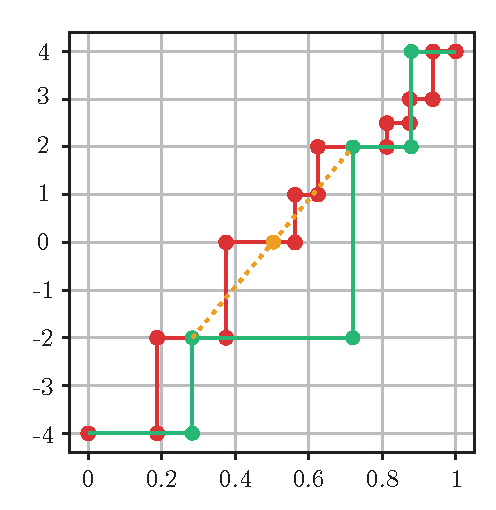
\includegraphics[width=0.5\linewidth]{gfx/heuristic.pdf}
\caption[The VaR-based heuristic.]{Visualization of the VaR-based heuristic. Quantile function of the exact distribution (unknown to the model) is shown in red and the VaR estimates at selected $\alpha$-levels are shown in green. Let's say we now want to know $y$ where $\var_y = 0$. We use linear interpolation between the nearest known VaRs, shown in orange. In this case the interpolation estimate is $y=0.5$.}
\label{fig:heuristic}
\end{figure}


\begin{algorithm}[!p]
\caption{CVaR Q-learning policy}\label{alg:varbasedpolicy}
\begin{algorithmic}
    \STATE \textbf{input:} $\alpha$, converged $V, C$
    		
	\STATE $x = x_0$
	\STATE $a = \argmax_a C(x, a, \alpha)$
	\STATE $s = V(x, a, y)$
	\WHILE{$x$ is not terminal}
	\STATE $\mathbf{d}_a = \text{extractDistribution}\bround{C(x', a, \bigcdot), \mathbf{y}}$ for each $a$
	\STATE $a = \argmax_a \text{expMinInterp}(s, \mathbf{d}, V(x', a, \bigcdot), \mathbf{y})$
	\STATE Take action $a$, observe $r, x'$
	\STATE $s = \dfrac{s-r}{\gamma}$
	\STATE $x = x'$
	\ENDWHILE

\hrulefill

	\STATE \comment{Compute $\mathbb{E}\left[(\mathbf{d}_a-s)^-\right]$ with linear interpolation}
	\STATE \textbf{function} expMinInterp  
\bindent
    \STATE \textbf{input:} $s$, vectors $\mathbf{d}, \mathbf{V}, \mathbf{y}$
    \STATE $z = 0$
    \FOR{$i \in \braces{1, ..., |\mathbf{y}|}$}
    	\IF{$S < V_i$}
		\STATE \textbf{break}
		\ENDIF
		\STATE $z = z + d_i\cdot(y_i - y_{i-1})$
	\ENDFOR
	
	\STATE $p_{\text{last}} = \dfrac{s - V_{i-1}}{V_{i}-V_{i-1}}(y_i - y_{i-1})$
	\STATE $z = z + d_i \cdot p_{\text{last}}$
	
	\STATE \textbf{output} $z$
\eindent
\end{algorithmic}
\end{algorithm}

\clearpage

%To side-step this issue, we bring the VaR-based improvement closer to CVaR Value Iteration and use it only in a one-step context. In each step, we compute the next $y$ as $F_{Z(x)}(\dfrac{s-r}{\gamma})$, which we extract from our VaR estimate $V$. Since we don't have access to the exact VaR for each $y \in [0,1]$ due to discretization, we use linear interpolaton as a heuristic. See \algref{varxibasedpolicy} for the full procedure.

%\begin{algorithm}
%\caption{CVaR Q-learning policy}\label{alg:varxibasedpolicy}
%\begin{algorithmic}
%    \STATE \textbf{input:} $\alpha$, converged $V, C$
%    		
%	\STATE $x = x_0$
%	\STATE $y = \alpha$
%	\WHILE{$x$ is not terminal}
%	\STATE $a = \argmax_a C(x, a, y)$
%	\STATE $s = V(x, a, y)$
%	\STATE Take action $a$, observe $r, x'$
%	\STATE $y = F_{Z(x')}(\dfrac{s-r}{\gamma})$
%	\STATE $x = x'$
%	\ENDWHILE
%\end{algorithmic}
%\end{algorithm}


%\begin{algorithm}
%\caption{Full CVaR Q-learning}
%\begin{algorithmic}
%    \STATE Initialize $V(x, a, y), C(x, a, y)$ for all $x\in\cX, a\in\cA, y\in\cY$ arbitrarily, and $C(x_\text{terminal}, \cdot, \cdot) = 0$
%    
%	\FOR{each episode}
%		
%	\STATE $x = x_0$
%	\STATE $y = \alpha$
%	\STATE $s = V(x, a, y)$
%	\WHILE{$x$ is not terminal}
%	\STATE Choose $a$ using a policy derived from $C, y$ (e.g. $\varepsilon$-greedy)
%	\STATE Take action $a$, observe $r, x'$
%	\STATE Update current estimates $V(x, a, y_i), C(x, a, y_i)$ (\algref{cvartd})
%	\STATE $y = F_{Z(x')}(\dfrac{s-r}{\gamma})$
%	\STATE $s = V(x, a, y)$
%	\STATE $x = x'$
%	\ENDWHILE
%	
%	\ENDFOR
%\end{algorithmic}
%\end{algorithm}


%*****************************************
%*****************************************
%*****************************************

\section{Experiments}\label{sec:qexperiments}
We use the same gridworld from \secref{vi:experiments} with $\delta=0.1$. Since the positive reward is very sparse, we chose to run CVaR Q-learning on a smaller environment of size $10\times15$. We trained the agent for 10,000 sampled episodes with learning rate $\beta=0.4$ that dropped each 10 episodes by a factor of 0.995. The used policy was $\varepsilon-$greedy and maximized expected value ($\alpha=1$) with $\varepsilon=0.5$. Notice the high value of $\varepsilon$. We found that lower $\varepsilon$ values led to overfitting the optimal expected value policy as the agent updated states out of the optimal path sparsly. This point will be elaborated further in the experimental section of the next chapter.

With said parameters, the agent was able to learn the optimal policies for different levels of $\alpha$. See \figref{qgrid} for learned policies and \figref{qhist} for Monte Carlo comparisons.

\begin{figure}[h]
\center
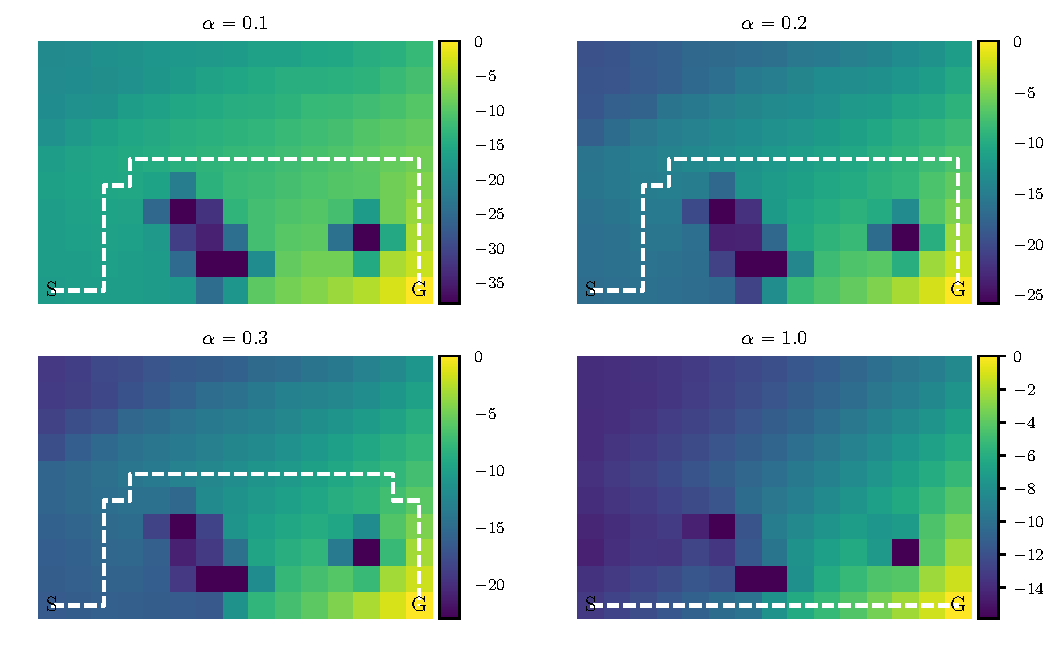
\includegraphics[width=\linewidth]{gfx/q_optimal_paths.pdf}
\caption[Grid-world CVaR Q-learning simulations.]{Grid-world Q-learning simulations. The optimal deterministic paths are shown together with CVaR estimates for given $\alpha$.}
\label{fig:qgrid}
\end{figure}


\begin{figure}[h]
\center
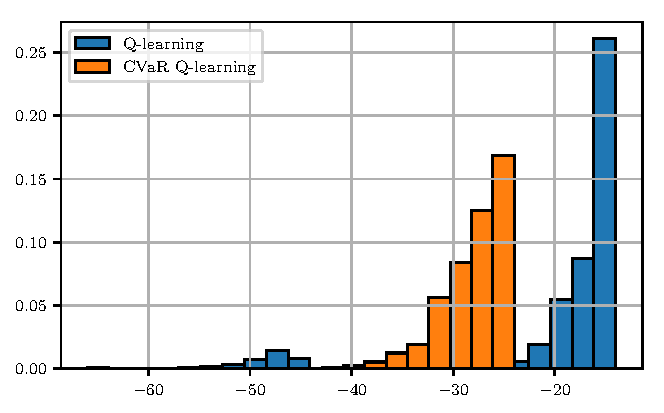
\includegraphics[width=0.8\linewidth]{gfx/sample_hist.pdf}
\caption[Grid-world CVaR Q-learning histograms.]{Histograms from 10000 runs generated by Q-learning and CVaR Q-learning with $\alpha=0.1$.}
\label{fig:qhist}
\end{figure}

The training was done with $N=50$ linearly-spaced atoms. We experimented with several discretization settings and didn't find many differences between log- and linearly-spaced points. Note that learning $\var$ and $\cvar$ for very low $\alpha$ values requires large number of samples and we found that extremely small atom values converged slowly.
\\
\\
\textit{Note on convexity:} Unlike CVaR Value Iteration, where we maintain convexity of the $y\cvar_y$ function with each update (given we started with convex estimates), in CVaR Q-learning we can break the convexity in each update for any atom. We experience this in practice as well as can be gauged from \figref{nonconvex}. Fortunately this fact does not break the update rule, since the targets we use to update $C$ as well as $V$ do not have to be ordered.


\begin{figure}[h]
\center
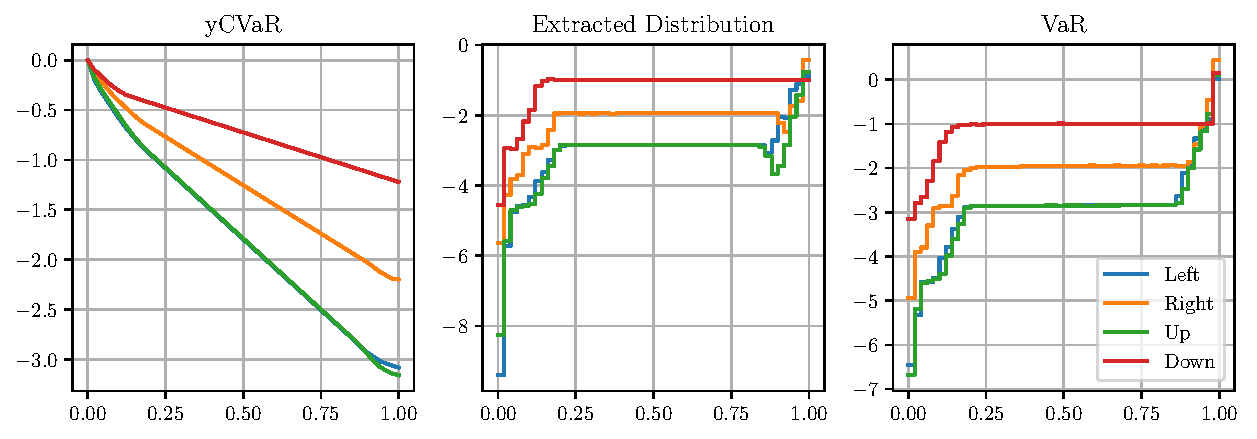
\includegraphics[width=\linewidth]{gfx/nonconvex.pdf}
\caption[Example CVaR Q-learning outputs.]{Learned $C, V$ estimates for a single state after 10000 episodes. Notice the nonconvexities visible from the extracted distribution plot. Both extracted distribution and VaR functions should be nondecreasing.}
\label{fig:nonconvex}
\end{figure}



%*****************************************
%*****************************************
%*****************************************
%*****************************************
%*****************************************


%************************************************
\chapter{Deep Q-learning with CVaR}\label{ch:dqn}
%************************************************

A big disadvantage of value iteration and Q-learning is the necessity to store a separate value for each state. When the size of the state-space is too large, we are unable to store the action-value representation and the algorithms become intractable. To overcome this issue, it is common to use function approximation together with Q-learning. \citet{mnih2015human} proposed the Deep Q-learning (DQN) algorithm and successfully trained on multiple different high-dimensional environments, resulting in the first artificial agent that is capable of learning a diverse array of challenging tasks.

In this chapter, we extend CVaR Q-learning to it's deep Q-learning variant and show the practicality and scalability of the proposed methods.

\section{Deep Q-learning}
The ultimate goal of artificial intelligence are agents that perform exhibit a wide range of skills. In the past, research was often focused on narrow AI, which was able to perform well on one particular task, but was unable to generalize to other tasks well. This has changed with the advent of deep learning \citep{krizhevsky2012imagenet}, that allowed us to train function approximators with the ability to generalize. Deep learning methods have become popular across all of machine learning, especially for supervised learning and vision.

\subsection{Deep Learning}

We include a short glossary of deep learning basics and terminology. There are much better sources to draw from and we refer the reader to \citet{goodfellow2016deep} for a comprehensive overview of the field.

Deep learning considers a particular class of parametrized function approximators called \textit{neural networks}. 
Neural networks are functions of the form $f_\theta(x) = f_n \circ f_{n-1} \circ\hdots\circ  f_1(x)$ where $f_i(x) = g_i(\theta_i x)$ with $g_i$ being usually a nonlinear function called the \textit{activation function} and $\theta_i$ is a parameter matrix. Every neural network has an input and output and several \textit{layers}, where a layer represents one matrix multiplication and application of an activation function $f_i(x)$.

The types of neural networks differ, from the simplest with straightforward matrix multiplication called multi layered perceprtons (MLP) to more complicated ones. Arguably the most important layer type that kick-started the popularity of deep learning is called a \textit{convolutional neural network} or CNN. Convolutional neural network consists of several (even hundreds in recent vision applications) so called convolutional layers and it's input is usually a 2D image. A convolutional layer consists of rectangular filters that look for increasingly abstract features by applying the same weight transformations over the whole image. The takeaway from us is that convolutional layers are able to learn from images, which is a fact we utilize in our experiments.

A necessary component of any deep learning algorithm is a loss function $\mathcal{L}$ to be minimized. The most common loss function being the mean squared error
\begin{equation*}
\mathcal{L} = \expval{(f_\theta(x) - \hat{y})^2}
\end{equation*}
with samples $\hat{y}$ representing the outputs drawn from a distribution of interest. 

The loss function is then minimized using Stochastic Gradient Descent, a stochastic version of the well-known gradient descent (see e.g. \citet{boyd2004convex}) where we perform each gradient step only using a subset of available samples. 
%\begin{equation}
%\theta_{t+1} = \theta - \beta\nabla_\theta \mathcal{L}
%\end{equation}
There exist many improved variants of SGD such as RMS-prop \cite{tieleman2012lecture} or Adam \citep{kingma2014adam}, that perform significantly better than the vanilla SGD algorithm and are often used in practice. See \citet{ruder2016overview} for a concise survey of the used algorithms.


\subsection{DQN}

Deep learning has also been succesfully applied to reinforcement learning. Q-learning have been used with function approximators in the past, however it suffers from instabilities during learning. In fact, it is well-known that Q-learning does not converge when used in conjunction with function approximators \citep{baird1995residual, sutton1998reinforcement} and this has been a problem in practice as well. \citet{mnih2015human} were able to stabilize the learning process by introducing two practical techniques. Firstly the model isn't learned online, meaning we see each example once, but instead a replay buffer is used to store transitions $(x, a, r, x')$ and these are later randomly sampled and used repeatedly for the updates. Secondly, a second network $Q'$ is used for computing the target values $r + \gamma Q'(x', a')$ and is only slowly updated towards $Q$. These improvements have helped to stabilize the learning greatly. See \algref{dqn} for the full procedure.

The DQN algorithm has been applied on the Atari Learning Environment \citep{bellemare13arcade}, a set of challenging and diverse tasks, with both inputs and outputs mirroring a human's experience of playing and learning the Atari games, and the same algorithm achieved human and superhuman-level performance on many of these games.

\begin{algorithm}
\caption{Deep Q-learning with experience replay}
\begin{algorithmic}\label{alg:dqn}

    \STATE Initialize replay memory $M$
    \STATE Initialize action-value function $Q$ with random weights $\theta$
    \STATE Initialize target action-value function $Q'$ with weights $\theta'=\theta$

    \FOR{each episode}
    \STATE $x=x_0$
	\WHILE{$x$ is not terminal}
	\STATE Choose $a$ using a policy derived from $Q$ ($\varepsilon$-greedy)
	\STATE Take action $a$, observe $r, x'$
	\STATE Store transition $(x, a, r, x')$ in $M$
	\STATE $x = x'$
	\STATE Sample random transitions $(x_j, a_j, r_j, x_j')$ from $M$
	\STATE Set $\cT Q_j=r_j + \gamma \max_{a'} Q'(x_j', a')$
    \STATE Perform a gradient step on $\bround{\cT Q_j - Q(x_j, a_j)}^2$ w.r.t. $\theta$
    \STATE Every $N_\text{target}$ steps set $\theta'=\theta$
	\ENDWHILE
	\ENDFOR
	
\end{algorithmic}
\end{algorithm}

\section{Distributional Reinforcement Learning with Quantile Regression}\label{sec:dqn:qrdqn}
Before we transition to CVaR Q-learning, we will mention the Quantile Regression DQN algorithm by \citet{dabney2017distributional}, which shares certain similarities with CVaR Q-learning.

In QR-DQN, the goal is to learn a distribution that minimizes the Wasserstein distance from the actual return distribution, since the distributional value iteration operator is a contraction in Wasserstein distance. 

The distributions are represented as $N$ discrete uniform atoms with probability $\frac{1}{N}$ and are parametrized with a value that, when learned correctly, represents the $\frac{y_{i}+y_{i+1}}{2}$ quantile, which is the Wasserstein minimizer.

The TD update rule for QR-DQN mimics the quantile estimation introduced in \chref{qlearning}:
\begin{equation*}
V_i(x, a) = V_i(x, a) + \beta \bsquare{1-\dfrac{1}{y_i}\indicator_{(V_i(x, a) \ge \cT V_j)}}
\end{equation*}
where $\cT V_j = r + \gamma V_j(x', a^*)$ and $a^*$ is selected as the action that maximizes the expected value in the next state. The target is created for each atom $y_j$ separately and differs from the one introduced in CVaR Q-learning.

The loss function reflects the asymmetry of the quantile and it is the standard quantile regression loss
\begin{equation}
\sum_{i=1}^{N} \expect_j\bsquare{(\cT V_j - V_i(x, a))(y_j - \indicator_{(V_i(x, a) \ge \cT V_j)})}
\end{equation}
See \figref{losses} for a visual comparison of loss functions used when finding expectations vs quantiles.

\begin{figure}[h]
\center
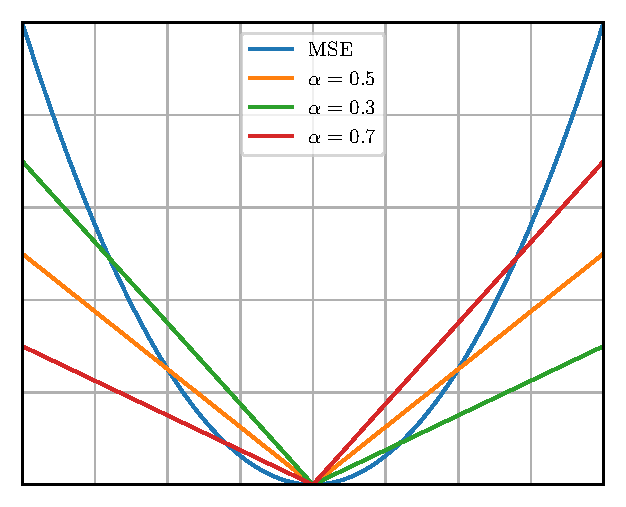
\includegraphics[width=0.6\linewidth]{gfx/losses.pdf}
\caption{Comparison of quantile loss function and Mean Squared Error.}
\label{fig:losses}
\end{figure}

The algorithm is then extended to it's deep Q-learning variant and verified empirically, which is a template we follow in the rest of this chapter.

\section{Deep CVaR Q-learning}
The transition from CVaR Q-learning to Deep CVaR Q-learning (CVaR DQN) follows the same principles as the one from Q-learning to DQN. Recall the TD update rule for CVaR Q-learning:
\begin{align*}
V(x, a, y_i) &= V(x, a, y_i) + \beta \expect_j\bsquare{1 - \dfrac{1}{y_i}\indicator_{(V(x, a, y_i) \ge r+\gamma d_j)}}\\
C(x, a, y_i) &= (1-\beta)C(x, a, y_i) + \beta\expect_j\bsquare{V(x, a, y_i) + \dfrac{1}{y_i}\bround{r+\gamma d_j - V(x, a, y_i)}^-}
\end{align*}
First significant change against DQN or QR-DQN is that we need to represent two separate values - one for $V$, one for $C$. As with DQN, we need to reformulate the updates as arguments minimizing some loss function.

\subsection{Loss functions}
The loss function for $V(x, a, y)$ is similar to QR-DQN loss in that we wish to find quantiles of a particular distribution. The target distribution however is constructed differently - in CVaR-DQN we extract the distribution from the $y\cvar_y$ function of the next state $\cT V = r + \gamma \mathbf{d}$.
\begin{equation}
\mathcal{L}_{\var}=\sum_{i=1}^{N} \expect_j\bsquare{(r + \gamma d_j - V_i(x, a))(y_j - \indicator_{(V_i(x, a) \ge r + \gamma d_j)})}
\end{equation}
where $d_j$ are atoms of the extracted distribution.

Constructing the CVaR loss function consists of transforming the running mean into MSE, again with the transformed distribution atoms $d_j$
\begin{equation}
\mathcal{L}_{\cvar}=\sum_{i=1}^{N} \expect_j\bsquare{\bround{V_i(x, a) + \frac{1}{y_i} \bround{r + \gamma d_j - V_i(x, a)}^- - C_i(x, a)}^2}
\end{equation}


Putting it all together, we are now able to construct the full CVaR-DQN loss function in \algref{cvardqnloss}.

\begin{algorithm}
\caption{Deep CVaR Loss function}
\begin{algorithmic}\label{alg:cvardqnloss}

    \STATE \textbf{input:} $x, a, x', r$
    \bindent
    \FOR{each $y_i$ }
	\STATE $C(x', y_i) = \max_{a'} C(x', a', y_i)$
	\ENDFOR
	
	\STATE $\mathbf{d}= \text{extractDistribution}\bround{C(x', \mathbf{y})}$

	
	\STATE $\mathcal{L}_{\var}=\sum_{i=1}^{N} \expect_j\bsquare{(r + \gamma d_j - V_i(x, a))(y_j - \indicator_{(V_i(x, a) \ge r + \gamma d_j)})}$
	\STATE $\mathcal{L}_{\cvar}=\sum_{i=1}^{N} \expect_j\bsquare{\bround{V_i(x, a) + \frac{1}{y_i} \bround{r + \gamma d_j - V_i(x, a)}^- - C_i(x, a)}^2}$
	\eindent
	\RETURN $\mathcal{L}_{\var} + \mathcal{L}_{\cvar}$
	
\end{algorithmic}
\end{algorithm}

Combining the loss functions with the full DQN algorithm, we get the full CVaR-DQN with experience replay, see \algref{cvardqn}. Note that we also utilize a target network $C'$ that is used for extraction of the target values, similarly to the original DQN. The network $V$ does not have a target network since the target is constructed independently of the value $V$.
\begin{algorithm}
\caption{Deep CVaR Q-learning with experience replay}
\begin{algorithmic}\label{alg:cvardqn}

    \STATE Initialize replay memory $M$
    \STATE Initialize the VaR function $V$ with random weights $\theta_v$
    \STATE Initialize the CVaR function $C$ with random weights $\theta_c$
    \STATE Initialize target CVaR function $C'$ with weights $\theta_c'=\theta_c$

    \FOR{each episode}
    \STATE $x=x_0$
	\WHILE{$x$ is not terminal}
	\STATE Choose $a$ using a policy derived from $C$ ($\varepsilon$-greedy)
	\STATE Take action $a$, observe $r, x'$
	\STATE Store transition $(x, a, r, x')$ in $M$
	\STATE $x = x'$
	\STATE Sample random transitions $(x_j, a_j, r_j, x_j')$ from $M$
	\STATE Build the loss function $\mathcal{L}_{\var} + \mathcal{L}_{\cvar}$ (\algref{cvardqnloss})
    \STATE Perform a gradient step on $\mathcal{L}_{\var} + \mathcal{L}_{\cvar}$ w.r.t. $\theta_v, \theta_c$
    \STATE Every $N_\text{target}$ steps set $\theta_c'=\theta_c$
	\ENDWHILE
	\ENDFOR
	
\end{algorithmic}
\end{algorithm}

%*****************************************
\newpage

\section{Experiments}

To test the approach in a complex setting, we applied the CVaR DQN algorithm to environments with visual state representation, which would be intractable for Q-learning without approximation. 

\subsection{Atari}
We ran several experiments on the Arcade Learning Environment \citep{bellemare13arcade}, which is used as a benchmark for many Deep Q-learning algorithms. The CVaR-DQN algorithm was able to learn reasonable policies with similar speed and performance as the original DQN algorithm. Unfortunately, due to the inherent determinism of the ALE, we didn't find significant differences between policies optimizing $\cvar_\alpha$ on different confidence levels, which led us to the construction of a new visual environment more suitable to risk-sensitive decision making.

\subsection{Ice Lake}
Ice Lake is a visual environment specifically designed for risk-sensitive decision making. Imagine you are standing on an ice lake and you want to travel fast to a point on the lake. Will you take the a shortcut and risk falling into the cold water or will you be more patient and go around? This is the basic premise of the environment which is visualized in \figref{icelake}.

The agent has five discrete actions, namely go \textit{Left, Right, Up, Down} and \textit{Noop}. These correspond to moving in the respective directions or no operation. Since the agent is on ice, there is a sliding element in the movement - this is mainly done to introduce time dependency and makes the environment a little harder. The environment is updated thirty times per second.

The agent recieves a negative reward of -1 per second, 100 if he reaches the goal unharmed and -50 if the ice breaks, then the episode ends. This particular choice of reward leads to about a $10\%$ chance of breaking the ice when taking the shortcut and it is still advantageous for a risk-neutral agent to take the dangerous path.

\begin{figure}[h]
\center

\includegraphics[width=0.3\linewidth]{gfx/icelake_start.png}
\caption{The Ice Lake environment. The agent is black and his target is green. The blue ring represents a dangerous area with risk of breaking the ice. \todo{outline, paths}}
\label{fig:icelake}
\end{figure}

\subsection{Network Architecture}
During our experiments we used the original DQN architecture, including the visual preprocessing trick used in \citet{mnih2015human}.

Firstly, the input images are scaled to $84\times84$ pixels and converted to greyscale to ease memory requirements. In many visual environments, a single image cannot capture the full state information - for example to track the velocity of different objects necessitates to track the objects in time. This problem is solved by concatenating 4 subsequent images which are then used as a single state representation. The input for each state is then of size $84\times84\times4$.

The neural network used in DQN inputs the state representation and outputs a value for each discrete action. The first hidden layer convolves 32 filters of $8\times8$ with stride 4 with the input image and applies a rectifier nonlinearity activation function \citep{jarrett2009best}. The second hidden layer convolves 64 filters of $4\times4$ with stride 2, again followed by a rectifier nonlinearity. This is followed by a third convolutional layer that convolves 64 filters of $3\times3$ with stride 1 followed by a rectifier. The final hidden layer is fully-connected and consists of 512 rectifier units. The output layer is a fully-connected linear layer with a single output for each valid action.
\\
\\
The architecture used in our experiments differs slightly from the original one used in DQN. In our case the output is not a single value but instead a vector of values for each action, representing $\cvar_y$ or $\var_y$ for the different confidence levels $y$. This issue is reconciled by having the output of shape $|\cA|\times N$ where $N$ is the number of atoms we want to use and $|\cA|$ is the action space size.

Another important difference is that we must work with two outputs - one for $C$, one for $V$. We have experimented with two separate networks (one for each value) and also with a single network differing only in the last layer. This approach may be advantageous, since we can imagine that the information required for outputting correct $V$ or $C$ is similar. Furthermore, having a single network instead of two eases the computation requirements.

We tested both approaches and since we didn't find significant performance differences, we settled on the faster version with shared weights. We also used 256 units instead of 512 to ease the computation requirements.

The implementation was done in Python and the neural networks were built using Tensorflow \citep{abadi2016tensorflow} as the framework of choice for gradient descent. The code was based on OpenAi baselines \citep{baselines}, an open-source DQN implementation.

\subsection{Parameter Tuning}
During our experiments, we tested mostly with $\alpha=1$ so as to find reasonable policies quickly. We noticed that the optimal policy with respect to expected value was found fast and other policies were quickly abandoned due to the character of $\epsilon$-greedy exploration. Unlike standard Reinforcement Learning, the CVaR optimization approach requires to find not one but in fact a continuous spectrum of policies - one for each possible $\alpha$. 
This fact, together with the exploration-exploitation dilemma, contributes to the difficulty of learning the correct policies.

After some experimentation, we settled on the following points: 

\begin{itemize}
\item The training requires a higher value of $\epsilon$ than DQN. While in DQN the final $\epsilon$ used during vast majority of the algorithm is 0.01, we settled on $0.3$ as a reasonable value with the ability to explore faster, while making the learned trajectories exploitable.

\item Training with a single policy is insufficient in larger environments. Instead of maximizing $\cvar$ for $\alpha=1$ as in our CVaR Q-learning experiments, we change the value $\alpha$ for each episode.

\item The random initialization used in deep learning has a detrimental effect on the initial distribution estimates, due to the way how the target is constructed and this sometimes leads to the introduction of extreme values during the initial training. We have found that clipping the gradient norm helps to mitigate these problems and overall helps with the stability of learning.
\end{itemize}

See ***appendix*** for a full parameter ****description. ** adam

\subsection{Results}

With the tweaked parameters, the algorithm was able to converge and learn both the optimal expected value policy and the risk-sensitive policy. See \todo{video or something also atari of something ?}

Although we tested with the vanilla version of DQN, we expect that all the DQN improvements such as experience replay \citep{hessel2017rainbow}, dueling \citep{wang2015dueling}, parameter noise \citep{plappert2017parameter} and others (combining the improvements matters, see \citep{hessel2017rainbow}) should have a positive effect on the learning performance. Another practical improvement may be the introduction of Huber loss, similarly to QR-DQN.

%*****************************************
%*****************************************
%*****************************************
%*****************************************
%*****************************************


%\part{Conclusion}\label{pt:end}
%************************************************
\chapter{Conclusion}\label{ch:conclusion}
%************************************************

\citet{bauerle2011markov}
\citet{bellemare2017distributional}
\citet{chow2015risk}
\citet{dabney2017distributional}
\citet{garcia2015comprehensive}
\citet{majumdar2017should}
\citet{morimura2010nonparametric}
\citet{morimura2012parametric}
\citet{pflug2016time}
\citet{rockafellar2000optimization}
\citet{rockafellar2002conditional}
\citet{majumdar2017should}
\citet{leike2017ai}
\citet{amodei2016concrete}
\citet{shapiro2013kusuoka}
\citet{artzner1999coherent}
\citet{tamar2015policy}
\citet{sutton1998reinforcement}
\citet{watkins1992q}
\citet{bellman1957markovian}
\citet{tsitsiklis1994asynchronous}
\citet{boyd2004convex}
\citet{kreyszig1989introductory}
\citet{koenker2001quantile}
\citet{basel2013fundamental}
\citet{mnih2015human}
\citet{silver2017mastering}
\citet{bahdanau2014neural}
\citet{krizhevsky2012imagenet}










%*****************************************
%*****************************************
%*****************************************
%*****************************************
%*****************************************



% ********************************************************************
% Backmatter
%*******************************************************
\appendix
%\renewcommand{\thechapter}{\alph{chapter}}
%\cleardoublepage
%\part{Appendix}
%************************************************
\chapter{Appendix}
%************************************************
%CVaR Value Iteration Linear Program:
\begin{equation}\label{eqn:cvarvilp}
\begin{split}
\min_{\xi, I_{x'}} \dfrac{1}{y} &\sum_{x'} p(x'|x, a) I_{x'}
\\
\textup{s.t.} \quad
&0 \le \xi \le \dfrac{1}{y}\\
&I_{x'} \ge y_iC(x,y_{i})+\frac{y_{i+1}C(x,y_{i+1})-y_iC(x,y_{i})}{y_{i+1}-y_i}(y\xi(x')-y_i) &\forall i, \forall x'\\
&\sum_{x'} p(x'|x, a)\xi(x') = 1 &\forall x'
\end{split}
\end{equation}
\begin{table}[h]
\centering
\caption{CVaR DQN training parameters}
\label{dqnparams}
\begin{tabular}{l|l|p{7cm}}
\textbf{Hyperparameter}         & \textbf{Value} & \textbf{Description}                                                                    \\\hline
minibatch size                  & 32             & Number of samples over which each SGD update is computed.                               \\
replay memory size              & 300000         & SGD updates are sampled from this number of recent frames.                              \\
target network update frequency & 5000           & The frequency $N_{\text{target}}$ with which the target network $C'$ is updated.        \\
$\gamma$                        & 0.99           & Discount Factor.                                                                        \\
update frequency                & 4              & We perform single gradient step each 4 frames.                                          \\
learning rate                   & 0.0001         & We use Adam with $\beta_1=0.9, \beta_2=0.999, \epsilon=$1e-8.                           \\
initial exploration             & 1.             & Initial value of $\epsilon$ in $\epsilon$-greedy.                                       \\
final exploration               & 0.3            & Initial value of $\epsilon$ in $\epsilon$-greedy.                                       \\
final exploration frame         & 1000000        & $\epsilon$ is linearly annealed from initial to final value over this number of frames. \\
training starts                 & 10000          & First update is performed after what number of steps.                                   \\
number of atoms                 & 100            & Number of uniformly spaced atoms to estimate quantiles.                                 \\
gradient norm clipping          & 10             & We clip the gradient if it's norm exceeds this value.                                  
\end{tabular}
\end{table}
%********************************************************************
% Other Stuff in the Back
%*******************************************************
\cleardoublepage%********************************************************************
% Bibliography
%*******************************************************
% work-around to have small caps also here in the headline
% https://tex.stackexchange.com/questions/188126/wrong-header-in-bibliography-classicthesis
% Thanks to Enrico Gregorio
\defbibheading{bibintoc}[\bibname]{%
  \phantomsection
  \manualmark
  \markboth{\spacedlowsmallcaps{#1}}{\spacedlowsmallcaps{#1}}%
  \addtocontents{toc}{\protect\vspace{\beforebibskip}}%
  \addcontentsline{toc}{chapter}{\tocEntry{#1}}%
  \chapter*{#1}%
}
\printbibliography[heading=bibintoc]

% Old version, will be removed later
% work-around to have small caps also here in the headline
%\manualmark
%\markboth{\spacedlowsmallcaps{\bibname}}{\spacedlowsmallcaps{\bibname}} % work-around to have small caps also
%\phantomsection
%\refstepcounter{dummy}
%\addtocontents{toc}{\protect\vspace{\beforebibskip}} % to have the bib a bit from the rest in the toc
%\addcontentsline{toc}{chapter}{\tocEntry{\bibname}}
%\label{app:bibliography}
%\printbibliography

\cleardoublepage%*******************************************************
% Declaration
%*******************************************************
\refstepcounter{dummy}
\pdfbookmark[0]{Declaration}{declaration}
\chapter*{Declaration}
\thispagestyle{empty}
Put your declaration here.
\bigskip

\noindent\textit{\myLocation, \myTime}

\smallskip

\begin{flushright}
    \begin{tabular}{m{5cm}}
        \\ \hline
        \centering\myName \\
    \end{tabular}
\end{flushright}

\cleardoublepage\pagestyle{empty}

\hfill

\vfill


\pdfbookmark[0]{Colophon}{colophon}
\section*{Colophon}
This document was typeset using the typographical look-and-feel \texttt{classicthesis} developed by Andr\'e Miede and Ivo Pletikosić.
The style was inspired by Robert Bringhurst's seminal book on typography ``\emph{The Elements of Typographic Style}''.
\texttt{classicthesis} is available for both \LaTeX\ and \mLyX:
\begin{center}
\url{https://bitbucket.org/amiede/classicthesis/}
\end{center}
Happy users of \texttt{classicthesis} usually send a real postcard to the author, a collection of postcards received so far is featured here:
\begin{center}
\url{http://postcards.miede.de/}
\end{center}
Thank you very much for your feedback and contribution.

\bigskip

\noindent\finalVersionString

%Hermann Zapf's \emph{Palatino} and \emph{Euler} type faces (Type~1 PostScript fonts \emph{URW
%Palladio L} and \emph{FPL}) are used. The ``typewriter'' text is typeset in \emph{Bera Mono},
%originally developed by Bitstream, Inc. as ``Bitstream Vera''. (Type~1 PostScript fonts were made
%available by Malte Rosenau and
%Ulrich Dirr.)

%\paragraph{note:} The custom size of the textblock was calculated
%using the directions given by Mr. Bringhurst (pages 26--29 and
%175/176). 10~pt Palatino needs  133.21~pt for the string
%``abcdefghijklmnopqrstuvwxyz''. This yields a good line length between
%24--26~pc (288--312~pt). Using a ``\emph{double square textblock}''
%with a 1:2 ratio this results in a textblock of 312:624~pt (which
%includes the headline in this design). A good alternative would be the
%``\emph{golden section textblock}'' with a ratio of 1:1.62, here
%312:505.44~pt. For comparison, \texttt{DIV9} of the \texttt{typearea}
%package results in a line length of 389~pt (32.4~pc), which is by far
%too long. However, this information will only be of interest for
%hardcore pseudo-typographers like me.%
%
%To make your own calculations, use the following commands and look up
%the corresponding lengths in the book:
%\begin{verbatim}
%    \settowidth{\abcd}{abcdefghijklmnopqrstuvwxyz}
%    \the\abcd\ % prints the value of the length
%\end{verbatim}
%Please see the file \texttt{classicthesis.sty} for some precalculated
%values for Palatino and Minion.
%
%    \settowidth{\abcd}{abcdefghijklmnopqrstuvwxyz}
%    \the\abcd\ % prints the value of the length

% ********************************************************************
% Game Over: Restore, Restart, or Quit?
%*******************************************************
\end{document}
% ********************************************************************
